\documentclass[11pt]{article}
\usepackage[margin=1in]{geometry}
\usepackage{amsmath,amssymb,amsthm}
\usepackage{graphicx,booktabs,array}
\usepackage{newtxtext}
\usepackage[subscriptcorrection]{newtxmath}
\usepackage[round,authoryear]{natbib}
\usepackage{xr}
\usepackage[hyphens]{url}
\emergencystretch=3em
\let\usc\_
\renewcommand{\_}{\usc\allowbreak}
\externaldocument[M-]{main}

\newtheorem{theorem}{Theorem}
\newtheorem{proposition}{Proposition}
\newtheorem{lemma}{Lemma}
\newtheorem{corollary}{Corollary}
\renewcommand{\thetheorem}{S\arabic{theorem}}
\renewcommand{\theproposition}{S\arabic{proposition}}
\renewcommand{\thelemma}{S\arabic{lemma}}
\renewcommand{\thecorollary}{S\arabic{corollary}}
\renewcommand{\thesection}{S\arabic{section}}
\renewcommand{\thefigure}{S\arabic{figure}}
\renewcommand{\thetable}{S\arabic{table}}
\renewcommand{\theequation}{S\arabic{equation}}
\renewcommand{\proofname}{Proof}

\newcommand{\pr}{\mathrm{pr}}
\newcommand{\LC}{\mathcal{L}}
\newcommand{\var}{\mathrm{var}}

\title{Supplementary material for `Latent coverage from noisy calibration'}
\author{Kun Woo Park}
\date{}

\begin{document}
\maketitle

\noindent Equation, theorem, table and section numbers without the prefix S refer to the main paper. The sections follow the order of the main paper, after a section of preliminaries. Each numerical statement says how it is supported: proved, certified in ball arithmetic, computed in double precision, or found by an exploratory search; \S~\ref{sec:s-cert} keeps these levels apart, and \S~\ref{sec:s-open} records a conjecture that no result uses. Table~\ref{tab:s-roadmap} shows where each result of the main paper is supported.

\begin{table}[h]
\centering
\caption{Where the results of the main paper are supported}
\label{tab:s-roadmap}
\footnotesize
\begin{tabular}{>{\raggedright\arraybackslash}p{0.36\textwidth}>{\raggedright\arraybackslash}p{0.27\textwidth}>{\raggedright\arraybackslash}p{0.27\textwidth}}
\toprule
main-paper result & supplement & support \\
\midrule
Proposition~\ref{M-prop:general} at both ends; one end is not enough & \S~\ref{sec:s-general} & proved \\
Theorem~\ref{M-thm:classes}(i), symmetric unimodal noise & \S~\ref{sec:s-general}, Proposition~\ref{prop:su-exact} & proved \\
Theorem~\ref{M-thm:classes}(ii), mean-zero log-concave noise & \S~\ref{sec:s-general} & proved; constants certified in ball arithmetic \\
Theorem~\ref{M-thm:classes}(iii), mean-zero unimodal noise & \S~\ref{sec:s-general} & proved \\
Proposition~\ref{M-prop:latentshape} & \S~\ref{sec:s-general} & proved; examples in closed form \\
Theorem~\ref{M-prop:unknown}; ranks of Table~\ref{M-tab:map} & \S~\ref{sec:s-ranks} & proved; ranks computed exactly \\
Proposition~\ref{M-prop:fail}; stress-test reliabilities & main text; \S~\ref{sec:s-sim} & proved; exact binomial values and simulation \\
Theorem~\ref{M-thm:small} & \S~\ref{sec:s-gauss}; constants \S~\ref{sec:s-cert} & proved; $c_q$ certified in ball arithmetic \\
feasibility bound and the $1.16\%$ and $0.22\%$ widenings & \S~\ref{sec:s-gauss}, feasibility; shape of the radius & proved; $0.22\%$ in double precision \\
Theorems~\ref{M-thm:mean} and~\ref{M-thm:transition} & \S~\ref{sec:s-gauss} & proved; $\kappa^*_q$ in double precision \\
Corollary~\ref{M-cor:slack} & \S~\ref{sec:s-gauss}, \S~\ref{sec:s-cert} & proved; slack intervals certified \\
rules with known variances (\S~\ref{sec:s-hetero}) & \S\S~\ref{sec:s-ranks}, \ref{sec:s-gauss}, \ref{sec:s-hetero} & proved; computed radius in double precision \\
Table~\ref{M-tab:sameinfo} & \S~\ref{sec:s-sim} & simulation, exact conditional coverage \\
shift of the new residual (\S~\ref{M-sec:discussion}) & \S~\ref{sec:s-shift} & proved \\
\bottomrule
\end{tabular}
\end{table}

\section{Preliminaries}\label{sec:s-prelim}

\emph{Notation.} The noise is $e$, and $\mathrm{e}$ is the base of the natural logarithm. A few symbols are reused with a local meaning, stated where they appear: $\ell$ is $\log q$ in \S~\ref{sec:s-general} and the length of a segment in \S~\ref{sec:s-cert}; $k$ is a rank, except in the parametrization $k = \beta L$ of \S~\ref{sec:s-general} and in $k_q(u)$; $h$ is $\min(1, q\mathrm{e}^{-y})$ in \S~\ref{sec:s-general} and a hazard or a grid step elsewhere; $\epsilon$ is a noise law, except as a small positive number in proofs of limits; $\delta$ is the reliability level, except as a small offset in constructions; $\phi$ is the standard normal density, $\phi_{\mathcal E}$ the one-end transfer of \S~\ref{sec:s-general} and $\varphi_\gamma$ its analogue in \S~\ref{sec:s-cert}; $x = D/t^2$ except in the proof of Proposition~\ref{prop:su-exact}.

\emph{Bi-log-concave laws.} $\mathcal B$ is the class of laws that are point masses or have a continuous distribution function $F$ with $\log F$ and $\log(1-F)$ concave \citep{dumbgen2017}; $\LC \subset \mathcal B$. The following facts are used throughout.
\begin{enumerate}
\item A law in $\mathcal B$ that is not a point mass has a positive density $f$ on the interior of its support, the hazard $f/(1 - F)$ is nondecreasing, $f/F$ is nonincreasing, and $f' \le f^2/F$ where $f$ is differentiable \citep{dumbgen2017}.
\item $\mathcal B$ is closed under convolution with a log-concave law. If $\log F_X$ is concave and $g$ is a log-concave density, $(t, y) \mapsto F_X(t - y)g(y)$ is log-concave on $\mathbb R^2$, so $F_{X+Y}(t) = \int F_X(t-y)g(y)\,dy$ is log-concave by the theorem of \citet{prekopa1973}, and likewise $1 - F_{X+Y}$.
\item $\mathcal B$ is closed under weak convergence \citep{saumard2019}: concavity of $\log F_n$ and $\log(1-F_n)$ passes to the limit at continuity points, and a limit that is not a point mass has no atom, because a concave function is continuous on the interior of its domain.
\item If $X$ has a continuous distribution function $F$ with $\log F$ concave and a finite mean, then $F\{E(X)\} \ge \mathrm{e}^{-1}$: $F(X)$ is uniform, so $E\{\log F(X)\} = -1$, and Jensen's inequality gives $\log F\{E(X)\} \ge E\{\log F(X)\}$. If also $\log(1 - F)$ is concave, $1 - F\{E(X)\} \ge \mathrm{e}^{-1}$ in the same way.
\end{enumerate}

\section{Coverage transfer for classes of noise laws}\label{sec:s-general}

This section proves the results of \S~\ref{M-sec:general}: the use of Proposition~\ref{M-prop:general} at both ends of the interval, the three parts of Theorem~\ref{M-thm:classes}, and Proposition~\ref{M-prop:latentshape}.

\subsection*{Proposition~\ref{M-prop:general} at both ends}

Let $\lambda_{\mathcal E}(p') = \sup\{q' : \Psi_{\mathcal E}(q') < p'\}$, which is the inverse of $\Psi_{\mathcal E}$ when $\Psi_{\mathcal E}$ is continuous and increasing, and let $\phi_{\mathcal E}(a) = 1 - \lambda_{\mathcal E}(1 - a)$. Both are nondecreasing.

Let $W \in \mathcal B$, let the noise be $e = \sigma\epsilon$ with $\epsilon$ in $\mathcal E$ and $\sigma > 0$, and let $a_R = \pr(W + e > 1)$ and $a_L = \pr(W + e < -1)$. The law of $Y = W - 1$ has $\log F_Y$ concave and $\pr(Y + e \le 0) = 1 - a_R$, and $e$ has a law in $\mathcal E$. By Proposition~\ref{M-prop:general}, $F_Y(0) \ge q'$ for every $q'$ with $\Psi_{\mathcal E}(q') < 1 - a_R$, so $\pr(W > 1) \le \phi_{\mathcal E}(a_R)$. The law of $-W - 1$ has a concave log distribution function, because $\log(1 - F_W)$ is concave and $F_W$ is continuous, and $-e$ has a law in $\mathcal E$; so $\pr(W < -1) \le \phi_{\mathcal E}(a_L)$. Hence, if $\phi_{\mathcal E}(a_L) + \phi_{\mathcal E}(a_R) \le 1 - q$ whenever $a_L + a_R \le 1 - p$, every $W \in \mathcal B$ with $\pr(|W + e| \le 1) \ge p$ has $\pr(|W| \le 1) \ge q$, for every noise law in $\mathcal E$ and every scale.

In the proof of Theorem~\ref{M-prop:unknown} this bound is applied to one unit at a time, so the noise laws may differ between units. Since $\phi_{\mathcal E}$ is nondecreasing, it suffices to check finitely many splits $(a_L, a_R)$, as in \S~\ref{sec:s-ball}. A certificate replaces $\lambda_{\mathcal E}$ by a smaller certified level, which only enlarges $\phi_{\mathcal E}$ and so keeps the bound valid.

\subsection*{One end is not enough}\label{sec:s-oneend}

No noisy level below $\Psi_{\mathcal E}(q)$ suffices. If $\Psi_{\mathcal E}(q) > p$, take $\epsilon$ in $\mathcal E$ with $E\{\min(1, q \mathrm{e}^{-\epsilon})\} > p$, let $a = \log(1/q)$, and let $W = 1 + s(a + \delta - E_1)$ with noise $s\epsilon$. As $s \to 0$ the left end contributes nothing, so the noisy coverage of $[-1, 1]$ tends to $E\{\min(1, q \mathrm{e}^{-\delta - \epsilon})\} > p$ for small $\delta > 0$, while the latent coverage tends to $q \mathrm{e}^{-\delta} < q$.

\subsection*{Proof of Theorem~\ref{M-thm:classes}(i): symmetric unimodal noise}

By the theorem of Khintchine, a law symmetric and unimodal about $0$ is that of $RU$, with $U$ uniform on $[-1, 1]$ and $R \ge 0$ independent of $U$. Hence $E\{\min(1, q \mathrm{e}^{-RU})\} = E\{g(R)\} \le \sup_r g(r)$, with $g(r) = E\{\min(1, q \mathrm{e}^{-rU})\}$, and uniform laws attain the supremum. With $\ell = \log q$,
\[
g(r) = q\,\frac{\sinh r}{r}\ (r \le -\ell), \qquad g(r) = \frac{\ell + r + 1 - q \mathrm{e}^{-r}}{2r}\ (r \ge -\ell).
\]
The first branch increases. On the second, $g'(r)$ has the sign of $d(r) = q \mathrm{e}^{-r}(1 + r) - (1 + \ell)$, which decreases, with $d(-\ell) = f(\ell) = \mathrm{e}^{2\ell}(1 - \ell) - 1 - \ell > 0$ because $f(0) = f'(0) = 0$ and $f''(\ell) = -4\ell\,\mathrm{e}^{2\ell} > 0$ for $\ell < 0$, and $d(r) \to -(1 + \ell) < 0$. So $g$ is maximal at the root $r$ of $d$, where $g(r) = \{1 + q \mathrm{e}^{-r}\}/2$.

Heavy tails are allowed: the $t_3$ and Cauchy laws are symmetric and unimodal, and for them the supremum over the scale is $0.90013$ and $0.9$ at $q = 0.9$ (numerical).

\subsection*{Symmetric unimodal noise: the exact two-sided level}

\begin{proposition}\label{prop:su-exact}
For symmetric unimodal noise, $\Psi = \Psi_{\mathcal E}$ is increasing and strictly convex on $(\mathrm{e}^{-1}, 1)$, and for $1/2 < p < 1$ and $\mathrm{e}^{-1} < q < 1$ the two-sided level is $p_{\mathcal E}(q) = \Psi(q)$: noisy coverage $p$ guarantees latent coverage $\lambda(p) = \Psi^{-1}(p)$ for every $W \in \mathcal B$ and every symmetric unimodal noise, possibly different between units, and no larger latent level is guaranteed, even for log-concave $W$.
\end{proposition}

\begin{proof}
Write $s = q \mathrm{e}^{-r}$ with $r$ the root of $d$, so that $\Psi(q) = (1 + s)/2$ and $s(1 + r) = 1 + \ell$. Since $\partial d/\partial r = -q r \mathrm{e}^{-r} < 0$, $r$ is differentiable in $q$; differentiating $s(1 + r) = 1 + \ell$ with $ds = s(dq/q - dr)$ gives $r s\,dr/dq = \ell/q$ and, using $\ell = s(1 + r) - 1$, $ds/dq = (rs - \ell)/(qr) = (1 - s)/(qr)$. Hence $\Psi'(q) = (1 - s)/(2qr) > 0$ and, after the same substitution,
\[
\Psi''(q) = \frac{(1 - s)\{1 - s(1 + r)^2\}}{2q^2 r^3 s}, \qquad 1 - s(1 + r)^2 = 1 - (1 + \ell)(1 + r).
\]
Let $x = 1 + \ell \in (0, 1)$ and $R = 1/x - 1$. As $d$ decreases on $(0, \infty)$, $r < R$ if and only if $d(R) < 0$, that is $\ell - R < 2\log x$, that is $k(x) = 2\log x - x + 1/x > 0$; and $k(1) = 0$, $k'(x) = -(1 - x)^2/x^2 < 0$. So $(1 + \ell)(1 + r) < 1$ and $\Psi'' > 0$. As $q \to 1$, $0 < r < R \to 0$ and $s \to 1$, so $\Psi$ extends continuously with $\Psi(1) = 1$, and $\Psi(q) \to 1/2$ as $q \downarrow \mathrm{e}^{-1}$.

The inverse $\lambda$ is therefore increasing and concave on $[1/2, 1]$, and $\phi(a) = 1 - \lambda(1 - a)$ is nondecreasing and convex on $[0, 1/2]$ with $\phi(0) = 0$, hence superadditive: $\phi(a_L) + \phi(a_R) \le \phi(a_L + a_R)$. By Proposition~\ref{M-prop:general}, letting the latent level increase to $\lambda(1 - a)$, an end with noisy failure probability $a$ has latent failure probability at most $\phi(a)$; the left end uses the negated noise, again symmetric unimodal. With $a_L + a_R \le 1 - p$ the latent failure probability is at most $\phi(1 - p) = 1 - \lambda(p)$, which is at most $1 - q$ when $p \ge \Psi(q)$.

Conversely, let $p < \Psi(q)$ and let $\epsilon$ be uniform on $[-r, r]$, with $r$ the maximizer. By the converse in Proposition~\ref{M-prop:general} there is an exponential tail $Y = a + \eta - E_1$, $\eta > 0$ small, with $F_Y(0) < q$ and $\pr(Y + \epsilon \le 0) > p$. For $\sigma > 0$ put $W = t + \sigma Y$, which is log-concave, and noise $\sigma\epsilon$. Then $\pr(|W| \le t) \le F_Y(0) < q$, while $\pr(|W + \sigma\epsilon| \le t) = \pr(Y + \epsilon \le 0) - \pr(Y + \epsilon < -2t/\sigma)$, which exceeds $p$ for small $\sigma$, since $\epsilon$ is bounded. The same construction with $q' > \lambda(p)$, for which $\Psi(q') > p$, shows that $\lambda(p)$ cannot be raised.
\end{proof}

At $q = 0.8$, $0.9$ and $0.95$ the two-sided levels are therefore $\Psi(q) = 0.8077245$, $0.9017873$ and $0.9504311$ (ball arithmetic, enclosures of width below $10^{-15}$), and noisy coverage $0.9$ guarantees exactly latent coverage $\lambda(0.9) = 0.8981432$, with $\Psi(0.8981) < 0.89996$ and $\Psi(0.8982) > 0.90005$. The same argument applies to any class $\mathcal E$ closed under scaling and negation whose one-sided function $\Psi_{\mathcal E}$ is convex; for Gaussian and mean-zero log-concave noise convexity is not proved, and the two-sided levels rest on the split certificates.

The split certificate of \S~\ref{sec:s-ball}, run for this class as an independent check (\texttt{split\_certificate\_su}), gives $p_{\mathcal E} \le 0.8078$, $0.9018$ and $0.9505$ at $q = 0.8$, $0.9$ and $0.95$, in agreement with Proposition~\ref{prop:su-exact}.

\subsection*{Proof of Theorem~\ref{M-thm:classes}(ii): mean-zero log-concave noise}

\emph{Reduction and parametrization.} Let $h(y) = \min(1, q \mathrm{e}^{-y})$, which is continuous, nonincreasing and $1$-Lipschitz. If $\epsilon$ is log-concave with mean zero, conditioning on $|\epsilon| \le M$ and recentring changes $E\{h(\epsilon)\}$ by at most $2\pr(|\epsilon| > M) + |E(\epsilon \mid |\epsilon| \le M)|$, which tends to zero; so it suffices to bound $E\{h(\epsilon)\}$ over log-concave laws on compact intervals with $E(\epsilon) \ge 0$, a larger class. By the localization theorem \citep{fradelizi2004} the supremum of this linear functional is attained at a point mass or at a law with density proportional to $\mathrm{e}^{\beta y}$ on a segment. A law with $E(\epsilon) > 0$ can be translated to mean zero without decreasing $E\{h(\epsilon)\}$, because $h$ is nonincreasing. So the supremum is over the point mass at $0$, where $h(0) = q$, and the mean-zero log-affine laws on segments. Write the latter as $\epsilon = L(V - \mu_k)$, $V$ on $[0, 1]$ with density proportional to $\mathrm{e}^{kv}$, $k = \beta L$, $\mu_k = E(V)$; then
\[
E\{h(\epsilon)\} = \frac{1}{Z_k}\Big\{\int_0^{v_c} \mathrm{e}^{kv}\,dv + q \mathrm{e}^{L\mu_k}\int_{v_c}^1 \mathrm{e}^{(k - L)v}\,dv\Big\}, \qquad v_c = \min\{1, \max(0, \mu_k + \ell/L)\},
\]
with $Z_k = \int_0^1 \mathrm{e}^{kv}\,dv$. For $|k| \ge 2$ we use the scale $\sigma = L/|k|$ and the truncated exponential form $\epsilon = \pm\sigma(\tau - m)$, $\tau$ standard exponential truncated to $[0, |k|]$, which includes $|k| = \infty$, the centred exponential laws $\pm\sigma(E - 1)$.

\emph{Upper bound on a box.} A branch and bound in Arb ball arithmetic, \texttt{uai.noise\_classes.lc\_certificate\_parallel}, bounds $E\{h(\epsilon)\}$ from above on boxes of $(k, L)$ for $|k| \le 2$ and of $(1/|k|, \sigma)$ for $|k| \ge 2$, splitting until each box is below the target. On a box the bound is
\[
E\{h(\epsilon)\} \le J(u) = \pr(\epsilon \le u) + q E\{e^{-\epsilon}; \epsilon > u\},
\]
which holds for every cut $u$ because $h(y) \le 1(y \le u) + q \mathrm{e}^{-y} 1(y > u)$. The cut is fixed at the kink of $h$ for the box centre, so that it does not depend on the parameters within the box; since $J'$ vanishes at the kink, the bound is tight to second order. Near $k = 0$, $Z_k$ and $\int_0^1 v \mathrm{e}^{kv}\,dv$ are evaluated by their series with a remainder bound. Box ends enter as exact doubles, and derived ends such as $1/|k|$ are rounded outward before they enter the ball computations.

\emph{Ends of the scale parameter.} The ends of the scale parameter are closed analytically.
\begin{enumerate}
\item For small $L$, $E\{h(\epsilon)\} \le q\,E(\mathrm{e}^{-\epsilon}) \le q \mathrm{e}^{L^2/24}$. With $K(s) = \log\int_0^1 \mathrm{e}^{sv}\,dv$ and $\epsilon = L(V - \mu_k)$, $\log E(\mathrm{e}^{-\epsilon}) = K(k - L) - K(k) + LK'(k) = \int_{k-L}^{k} (s - k + L) K''(s)\,ds \le L^2/24$, because $K''(s) = s^{-2} - \{2\sinh(s/2)\}^{-2}$, the variance of the law on $[0, 1]$ with density proportional to $\mathrm{e}^{sv}$, is at most its value $1/12$ at $s = 0$, as $x^{-2} - \sinh^{-2}x$ decreases in $|x|$. This improves on the bound $q \mathrm{e}^{L^2/8}$ of Hoeffding's lemma.
\item For large $L$, $h(y) \le 1$ for $y \le 4$ and $h(y) \le q \mathrm{e}^{-4}$ for $y > 4$, so $E\{h(\epsilon)\} \le \pr(\epsilon \le 4) + q \mathrm{e}^{-4}$. Here $\pr(\epsilon \le 4) = \pr(V \le \mu_k + 4/L) \le 1 - \mathrm{e}^{-1} + 4d/L$, by fact 4 of \S~\ref{sec:s-prelim} applied to $V$ and because the density of $V$ is at most $d = 2/(1 - \mathrm{e}^{-2})$ for $|k| \le 2$. The resulting bound $1 - \mathrm{e}^{-1} + 4d/L + q \mathrm{e}^{-4}$ is below the target once $L \ge L_{\rm big}$, which is found by enlarging $L$ until the inequality holds in ball arithmetic.
\item For small and large $\sigma$, the analogous bounds use $E(\mathrm{e}^{-\sigma\tau}) \le 1$, $E(\mathrm{e}^{\sigma\tau} \mid \tau \le |k|) \le (1 - \sigma)^{-1}$ and $m \ge 1 - 2/(e^2 - 1)$.
\end{enumerate}

\emph{Results.} At $q = 0.9$ the certificate gives $\Psi_{\mathcal E}(0.9) < 0.9052$; the largest certified bound for this target is $0.90519999990$, so the margin is about $10^{-10}$. The centred exponential with $\sigma = 0.11777$ gives $\Psi_{\mathcal E}(0.9) > 0.90517$; it gives $\Psi_{\mathcal E}(0.8942) > 0.9$ at $\sigma = 0.1259$.

For the two-sided levels, a partition of the noisy failure probability $a_L \in [0, (1 - p)/2]$ at the left end is proposed from the centred exponential values: on each interval $[a_0, a_1]$ the bound $\phi_{\mathcal E}(a_1) + \phi_{\mathcal E}(1 - p - a_0)$, evaluated at those values, uses at most half of the margin below $1 - q$, and the other half is left for the certificates. Every node $a$ is then certified by the branch and bound at a level $q_a$ below $\lambda_{\mathcal E}(1 - a)$; this certifies the noisy levels $0.9068$ and $0.906$ for latent level $0.9$, with $29$ and $41$ intervals, and noisy level $0.9$ for latent level $0.8935$, with $45$ intervals (\texttt{split\_certificate\_lc}).

Numerically the worst split puts the whole failure probability at one end, as for Gaussian and symmetric unimodal noise, so the two-sided level would be $\Psi_{\mathcal E}(0.9) = 0.905176$ (numerical). Numerically, along truncated exponential laws $\sigma(\tau - m)$ with a long right tail the supremum over the scale increases with the truncation length, to the centred exponential; for the reflected laws it decreases. These two statements are numerical and are not used.

\subsection*{Proof of Theorem~\ref{M-thm:classes}(iii): mean-zero unimodal noise}

Let $\epsilon$ have density $(1 - \rho)/a$ on $[-a, 0]$ and $\rho/b$ on $(0, b]$ with $b = (1 - \rho)a/\rho$ and $\rho \le 1/2$; it is unimodal with mean zero. Then $E\{h(\epsilon)\} \ge (1 - \rho)(1 + \ell/a)$, which tends to one as $\rho \to 0$ and $a \to \infty$, so $\Psi_{\mathcal E}(q) = 1$ and no noisy level below one transfers to any latent level.

\subsection*{Gaussian noise as a class}

For Gaussian noise $\Psi_{\mathcal E}(q) = \sup_{\sigma} E\{\min(1, q \mathrm{e}^{-\sigma Z})\}$, and Proposition~\ref{M-prop:general} recovers the sign of the constants of Lemma~\ref{lem:onesided}: $c_{p,q} \le 0$ if $\Psi_{\mathcal E}(q) < p$ and $c_{p,q} > 0$ if $\Psi_{\mathcal E}(q) > p$. At $q = 0.9$ the supremum is $0.900803$, at $\sigma = 0.0503$, in the slack interval $(0.90079, 0.901]$ of Corollary~\ref{M-cor:slack}.

\subsection*{Proof of Proposition~\ref{M-prop:latentshape}: unimodal latent laws}

The bound needs no shape. Given $W > 1$, the event $\epsilon \ge 0$ gives $W + \epsilon > 1$, and given $W < -1$ the event $\epsilon \le 0$ gives $W + \epsilon < -1$; both have probability at least $\beta_{\mathcal E}$, since $\mathcal E$ is closed under negation, so $1 - p \ge \pr(|W + \epsilon| > 1) \ge \beta_{\mathcal E}\pr(|W| > 1)$. For median-zero noise this is the bound of \citet{guille2024}; for mean-zero log-concave noise $\pr(\epsilon \ge 0) \ge \mathrm{e}^{-1}$ and $\pr(\epsilon \le 0) \ge \mathrm{e}^{-1}$ by fact 4 of \S~\ref{sec:s-prelim}, with equality for the centred exponential law $E_1 - 1$; for mean-zero unimodal noise $\beta_{\mathcal E} = 0$.

For the construction let $\epsilon$ have a law in $\mathcal E$, continuous at $0$, with $\pr(\epsilon \ge 0) = \beta < \beta_{\mathcal E} + \gamma'$; as $p > 1 - \beta_{\mathcal E}$, $(1 - p)/\beta < 1$ for small $\gamma'$. Let $\tau, \gamma'' > 0$ be small, $0 < \delta < 1$,
\[
s = (1 - p - \gamma'' - \tau)/\beta, \qquad m = 1 - s - \tau, \qquad A = 2s(1 + \delta/2)/\tau - 1,
\]
so that $s, m > 0$, and let $W$ have a density made of three pieces:
\begin{enumerate}
\item $m/2$ on $[-1, 1]$, the mass inside the interval;
\item $s/\delta$ on $(1, 1 + \delta]$, a thin layer just outside the right end;
\item $\tau/(A - 1)$ on $[-A, -1)$, a long light left tail that makes $E(W) = s(1 + \delta/2) - \tau(A + 1)/2 = 0$.
\end{enumerate}
For small $\tau$ the density is nondecreasing up to $1 + \delta$ and zero beyond it, so $W$ is unimodal. With noise $\sigma\epsilon$, the failures of $|W + \sigma\epsilon| \le 1$ come from the three pieces as follows. The left tail fails with probability at most $\tau$. The inside piece fails with probability $(m/2)\int_{-1}^{1} \pr(|w + \sigma\epsilon| > 1)\,dw$, which tends to $0$ as $\sigma \to 0$ by dominated convergence. The layer fails with probability at most $s\{\pr(\epsilon > -\delta/\sigma) + \pr(\epsilon < -2/\sigma)\}$: the second term, a large negative noise carrying the point past $-1$, tends to $0$, and the first tends to $\beta$ as $\sigma \to 0$ with $\delta/\sigma \to 0$, by continuity at $0$. So the noisy coverage tends to at least $1 - \tau - s\beta = p + \gamma'' > p$, while the latent coverage is $m = 1 - (1 - p - \gamma'' - \tau)/\beta - \tau$, within any $\gamma$ of $1 - (1 - p)/\beta_{\mathcal E}$ for small $\gamma'$, $\gamma''$ and $\tau$. If $\beta_{\mathcal E} = 0$, take $\beta < \gamma'$ and $s = 1 - \tau - \gamma$, so that the latent coverage is $m = \gamma$ while the noisy coverage tends to at least $1 - \tau - s\beta \ge 1 - \tau - \gamma' > p$ for small $\tau$ and $\gamma'$.

The noisy coverage of this law has a closed form: for a piece with uniform density on $[a, b]$, $\int_a^b F(c - w)\,dw = G(c - a) - G(c - b)$, where $F$ is the distribution function of the noise and $G$ an antiderivative, $G(y) = y\Phi(y/\sigma) + \sigma\phi(y/\sigma)$ for Gaussian noise. With $\tau = 10^{-4}$, $\delta = 10^{-3}\sigma$ and the noisy coverage set to $0.9$, the latent coverage is $0.870$, $0.820$, $0.807$ and $0.801$ at $\sigma = 0.1$, $0.03$, $0.01$ and $0.001$ for Gaussian noise, $0.876$, $0.822$, $0.807$ and $0.801$ for uniform noise of standard deviation $\sigma$, and $0.809$, $0.751$, $0.736$ and $0.729$ for the centred exponential noise $\sigma(E_1 - 1)$, against the limits $0.8$, $0.8$ and $1 - \mathrm{e}/10 = 0.72817\ldots$ (\texttt{experiments/e42\_unimodal\_boundary.py}).

\section{Finite-sample ranks}\label{sec:s-ranks}

This section gives the computations behind Theorem~\ref{M-prop:unknown} and Table~\ref{M-tab:map}, and the order-statistic level used by the rules with known variances.

\subsection*{Smallest valid ranks}

By Theorem~\ref{M-prop:unknown} the smallest valid rank is at most the smallest $k$ with $\pr\{{\rm Bin}(K, p) \le k - 1\} \ge 1 - \delta$ at $p = p_{\mathcal E}(q)$, and at least the smallest such $k$ at $p = \Psi_{\mathcal E}(q)$. At $q = 0.9$ and $\delta = 0.05$ a rank exists only if $1 - p^K \ge 0.95$, that is for $K \ge 29$ under Gaussian and symmetric unimodal noise, $K \ge 31$ under mean-zero log-concave noise and $K \ge 59$ at $p = 0.95$. Against the usual rank, with $p = 0.9$, the raise for Gaussian noise is $0$ at $K = 110$, $1$ at $K = 300$ and $10^3$, $3$ at $K = 3000$ and $8$ to $10$ at $K = 10^4$. The function \texttt{certified\_rank} returns this rank.

\emph{Unimodal latent laws.} The proof of Theorem~\ref{M-prop:unknown} uses only the transfer for one unit. With the transfer of Proposition~\ref{M-prop:latentshape}, which needs noisy level $1 - \beta_{\mathcal E}(1 - q)$, that is $(1 + q)/2$ for median-zero noise and $1 - (1 - q)/\mathrm{e}$ for mean-zero log-concave noise, it gives the ranks in the last two rows of Table~\ref{M-tab:map}: if $\pr(|W| \le s) < q$ then $\pr(|V_i| \le s) < 1 - \beta_{\mathcal E}(1 - q)$, for every latent law. These ranks are the smallest valid ones for unimodal latent laws with mean zero. Let $p < 1 - \beta_{\mathcal E}(1 - q)$ and take the construction in the proof of Proposition~\ref{M-prop:latentshape} with the layer mass $s$ chosen in $1 - q - \tau < s < (1 - \tau - p)/\beta$, which is possible for small $\tau$ and $\gamma'$. Then the latent coverage of $[-1, 1]$ is $m = 1 - s - \tau < q$, so $r = Q_q(|W|) > 1$, and the noisy coverage of $[-1, 1]$ tends to at least $1 - \tau - s\beta > p$, so $\pr(|V_i| < r) \ge \pr(|V_i| \le 1) > p$ for small $\sigma$. As in the proof of Theorem~\ref{M-prop:unknown}, the reliability of rank $k$ is then at most $\pr\{{\rm Bin}(K, p) \le k - 1\}$.

Proposition~\ref{M-prop:fail} is illustrated at an extremal law in \S~\ref{sec:s-sim}, with exact reliabilities up to $K = 10^6$.

\subsection*{An order-statistic level for known variances}

The computed radius and the shrunk threshold of \S~\ref{sec:s-hetero} use a level for the average noisy distribution function rather than a bound for each unit. Let $T = |V|_{(k)}$, let $\bar F$ be the average distribution function of the $|V_i|$, assumed continuous, and let $p_k$ be the $\delta$-quantile of the ${\rm Beta}(k, K+1-k)$ distribution.

\begin{proposition}\label{prop:beta}
If $k \ge Kp_k + 1$ then $\pr\{\bar F(T) \ge p_k\} \ge 1 - \delta$.
\end{proposition}

\begin{proof}[Proof of Proposition~\ref{prop:beta}]
$\bar F(T) < p_k$ exactly when $N = \#\{i : |V_i| < \bar F^{-1}(p_k)\} \ge k$. $N$ is a sum of independent indicators whose success probabilities average $p_k$, and $k - 1 \ge Kp_k$. By \citet{hoeffding1956}, $\pr(N \le k-1)$ is smallest when all success probabilities are equal. Hence $\pr(N \ge k) \le \pr\{{\rm Bin}(K, p_k) \ge k\} = \pr\{{\rm Beta}(k, K+1-k) \le p_k\} = \delta$.
\end{proof}

\section{Gaussian noise: the sharp radius and the location of the mean}\label{sec:s-gauss}

This section proves the results of \S~\ref{M-sec:mean}, for Gaussian noise $e \sim N(0, D)$, after scaling the threshold $t$ to $1$, with $x = D/t^2$ and $R_{p,q}$ defined by \eqref{M-eq:R}.

\subsection*{Reduction to log-affine laws}

Write $g_x(w) = \pr(|w + x^{1/2}Z| \le 1)$, so that the constraint in \eqref{M-eq:R} reads $E\{g_x(W)\} \ge p$, and let $\mathcal F$ be the family of point masses and of laws with density proportional to $\mathrm{e}^{\beta w}$ on a segment.

\begin{proposition}\label{prop:reduction}
$R_{p,q}(x) = \sup\{Q_q(|W|) : W \in \mathcal F,\ E\{g_x(W)\} \ge p\}$. The same holds for any continuous constraint kernel that vanishes at $\pm\infty$, in particular for the average kernel of \S~\ref{sec:s-hetero}.
\end{proposition}

The proof uses the localization theorem; over $\mathcal F$ the problem is a two-dimensional maximization of closed forms.

\begin{proof}[Proof of Proposition~\ref{prop:reduction}]
Since $\mathcal F \subset \LC$ it suffices to bound the supremum over $\LC$. Let $W \in \LC$ satisfy $E\{g_x(W)\} \ge p$ and let $s < Q_q(|W|)$, so that $\pr(|W| < s) \le q - \gamma$ for some $\gamma > 0$. Choose $M \ge s$ with $g_x(w) \le p$ for $|w| \ge M$, and let $W_M$ be $W$ conditioned on $|W| \le M$, which is log-concave. With $\varepsilon_M = \pr(|W| > M)$, the conditioning removes only mass on which the kernel is at most $p$, so
\[
E\{g_x(W_M)\} \ge \frac{p - p\varepsilon_M}{1 - \varepsilon_M} = p, \qquad \pr(|W_M| < s) \le \frac{q - \gamma}{1-\varepsilon_M} < q
\]
for $M$ large. On $[-M, M]$ the constraint function $g_x - p$ is continuous, and $\mu \mapsto -\mu(-s, s)$ is linear and upper semicontinuous for weak convergence because $(-s,s)$ is open. By the localization theorem \citep{kannan1995, fradelizi2004}, the supremum of this functional over the log-concave probability measures on $[-M, M]$ that satisfy $\int(g_x - p)\,d\mu \ge 0$ is attained at a point mass or at a law with log-affine density on a segment. Hence some member of $\mathcal F$ is feasible and has $\pr(|W| < s) < q$, that is, $Q_q(|W|) \ge s$. Since $s < Q_q(|W|)$ was arbitrary the claim follows. Only continuity of the kernel and its decay at infinity were used, so the argument applies to the average kernel $\bar g$ of \S~\ref{sec:s-hetero}.
\end{proof}

For $\beta > 0$ and $\sigma = x^{1/2}$, integration by parts gives
\begin{equation}\label{eq:closed}
\int_a^b \mathrm{e}^{\beta w}\Phi\Big(\frac{c-w}{\sigma}\Big)dw = \frac{1}{\beta}\Big[\mathrm{e}^{\beta w}\Phi\Big(\frac{c-w}{\sigma}\Big)\Big]_a^b + \frac{e^{\beta c + \beta^2\sigma^2/2}}{\beta}\Big\{\Phi\Big(\frac{b-c-\beta\sigma^2}{\sigma}\Big) - \Phi\Big(\frac{a-c-\beta\sigma^2}{\sigma}\Big)\Big\},
\end{equation}
so the constraint is a combination of normal distribution functions. For fixed slope and length, the translations $c$ of a member of $\mathcal F$ that satisfy the constraint form an interval, because $c \mapsto \pr(|W + c + e| \le 1)$ is log-concave \citep{prekopa1973}, and $c \mapsto \pr(|W + c| \le s)$ is log-concave, so $c \mapsto Q_q(|W + c|)$ is quasi-convex and is maximized at an end of that interval. Each end is found by a root-finding in $c$, and the quantile by a second root-finding, using \eqref{eq:closed}.

\subsection*{The one-sided problem}

Near each end of the interval the problem is one-sided. For $u > 0$ let $E_u$ be exponential with rate $u$, independent of $Z$, and for the exponential tail $b - E_u$ let
\[
m_u(b) = \pr(b - E_u + Z \le 0) = \Phi(-b) + \mathrm{e}^{-ub + u^2/2}\,\Phi(b - u),
\]
which is continuous and strictly decreasing in $b$. Let $b_u(p)$ solve $m_u(b) = p$, and write $v_q(u) = b_u(q) - u^{-1}\log(1/q)$ and $k_q(u) = u^{-1} - b_u(q)$; the law $b_u(q) - E_u$ has $q$-quantile $v_q(u)$ and mean $-k_q(u)$.

\begin{lemma}\label{lem:onesided}
Let $c_{p,q} = \sup\{F_Y^{-1}(q) : Y \in \LC,\ \pr(Y + Z \le 0) \ge p\}$ and $c_q = c_{q,q}$. Then $c_{p,q} = \sup_{u > 0}\{b_u(p) - u^{-1}\log(1/q)\}$, $c_q > 0$, and $q \mapsto c_q$ is nonincreasing. The same holds with $\mathcal B$ in place of $\LC$.
\end{lemma}

Ball arithmetic gives $c_{0.8} = 0.04607$, $c_{0.9} = 0.01906$ and $c_{0.95} = 0.00841$ (\S~\ref{sec:s-ball}). The proofs of Lemma~\ref{lem:onesided} and of Lemma~\ref{lem:meanonesided} below replace $Y$ by an exponential tail through a supergradient of $\log F_Y$ at its $q$-quantile, which keeps the quantile, the constraint and the bound on the mean.

\begin{proof}[Proof of Lemma~\ref{lem:onesided}]
Exponential tails are log-concave, which gives one inequality. Conversely, let $Y \in \LC$ with $\pr(Y + Z \le 0) \ge p$. If $Y = y_0$ is a point mass then $y_0 \le -\Phi^{-1}(p) = \lim_{u\to\infty}\{b_u(p) - u^{-1}\log(1/q)\}$. Otherwise $F = F_Y$ is continuous and $\log F$ is concave \citep{prekopa1973}. Let $v = F^{-1}(q)$ and $G(y) = F(v + y)$. The point $0$ is interior to $\{G > 0\}$, so the right derivative $u \ge 0$ of $\log G$ at $0$ is a supergradient, and $G(y) \le q \mathrm{e}^{uy}$ for all $y$. If $u = 0$ then $G \le q < 1$, which is impossible, so $u > 0$ and $G(y) \le \min(q\mathrm{e}^{uy}, 1)$, which is the distribution function of $b_0 - E_u$ with $b_0 = u^{-1}\log(1/q)$. Hence $Y' = v + b_0 - E_u$ lies stochastically below $Y$ and has $q$-quantile $v$, and
\[
p \le \pr(Y + Z \le 0) \le \pr(Y' + Z \le 0) = m_u(v + b_0).
\]
Since $m_u$ is decreasing, $v \le b_u(p) - b_0$. For monotonicity, let $q' > q$, let $Y$ be feasible at $(q', q')$ with $v = F_Y^{-1}(q')$, and put $\rho = (q' - q)/(1-q)$. Then $Y$ conditioned on $Y \ge F_Y^{-1}(\rho)$ is log-concave; over $\mathcal B$ it stays in $\mathcal B$, because $\log(F - \rho) = h(\log F)$ with $h(z) = \log(e^z - \rho)$ nondecreasing and concave, and the log survival function of the conditioned law is $\min\{0, \log(1-F) - \log(1-\rho)\}$, a minimum of concave functions. It satisfies the constraint at level $(q' - \rho)/(1-\rho) = q$, because the removed mass has noisy constraint value at most one, and has $q$-quantile $v$. Point masses have value $-\Phi^{-1}(q') < -\Phi^{-1}(q) \le c_q$. Finally, $c_q > 0$ because $v_q(u) = u^{-1}\log\{e^{u^2/2}\Phi(b_u - u) + \mathrm{e}^{u b_u}\Phi(-b_u)\} = u/2 + o(u)$ as $u \to 0$, where $b_u = b_u(q)$ and $u b_u \to \log(1/q)$.
\end{proof}

\subsection*{Theorem~\ref{M-thm:small}: the lower bound}

\begin{proof}[Proof of Theorem~\ref{M-thm:small}, lower bound]
Fix $\epsilon > 0$ and choose $u$ with $v_q(u) > c_q - \epsilon$. For $p' \in [q, (1+q)/2]$, $b_u(p') \ge b_{\min} > -\infty$. Let $Y = b_u(p') - E_u$ and $W = 1 + x^{1/2}Y$. With $\tau = 2x^{-1/2}$,
\[
\pr(|W+x^{1/2}Z| \le 1) = p' - \pr(Y + Z < -\tau) \ge p' - \eta_x, \qquad \eta_x = \mathrm{e}^{-u(\tau + b_{\min})/2} + \Phi\{-(\tau + b_{\min})/2\},
\]
by splitting the event $Y + Z < -\tau$ according to whether $Z < -(\tau + b_{\min})/2$. Take $p' = q + \eta_x$, which lies in $[q, (1+q)/2]$ for small $x$. Since $\pr(|W| \le s) \le F_W(s)$, $Q_q(|W|) \ge 1 + x^{1/2}\{b_u(q + \eta_x) - u^{-1}\log(1/q)\}$. As $\eta_x \to 0$ and $b_u$ is continuous, $\liminf_{x\to0}\{R_{q,q}(x) - 1\}/x^{1/2} \ge c_q - \epsilon$.
\end{proof}

\subsection*{Feasibility and the size of the widening}\label{sec:s-feasible}

The kernel $g_x(w) = \pr(|w + x^{1/2}Z| \le 1)$ is symmetric in $w$ and maximal at $w = 0$, so $E\{g_x(W)\} \le g_x(0) = 2\Phi(x^{-1/2}) - 1$ for every $W$. A latent law is therefore feasible at level $q$ only if $2\Phi(x^{-1/2}) - 1 \ge q$, that is $x^{1/2} \le 1/\Phi^{-1}\{(1+q)/2\}$. With Theorem~\ref{M-thm:small}, the widening $Q_q(|W|) - 1 \le c_q x^{1/2}$ is at most $c_q/\Phi^{-1}\{(1+q)/2\}$, which is $0.01906/1.6449 < 1.16\%$ at $q = 0.9$ for every $W \in \mathcal B$. The smaller bound $0.22\%$ for log-concave laws rests on the double-precision bounds of \S~\ref{sec:s-cert} (\S~\ref{sec:s-shape}).

\subsection*{A constraint on the mean}

\begin{lemma}\label{lem:meanonesided}
Let $\mathrm{e}^{-1} < q < 1$ and $\kappa \ge 0$. Then
\[
\sup\{F_Y^{-1}(q) : Y \in \mathcal B,\ E(Y) \le -\kappa,\ \pr(Y + Z \le 0) \ge q\} = L_q(\kappa) = \sup\{v_q(u) : u > 0,\ k_q(u) \ge \kappa\}.
\]
The function $L_q$ is positive and nonincreasing, and, for $q > 1/2$, $L_q(\kappa) = c_q$ for $\kappa \le \kappa^*_q$, where $\kappa^*_q$ is the largest value of $k_q$ on the compact set of maximizers of $v_q$, and $\kappa L_q(\kappa) \to \{1 - \log(1/q)\}/2$ as $\kappa \to \infty$. In double precision $\kappa^*_q = 6.81$, $20.18$ and $50.07$ at $q = 0.8$, $0.9$ and $0.95$.
\end{lemma}

\begin{proof}[Proof of Lemma~\ref{lem:meanonesided}]
For $q > 1/2$, $v_q$ is continuous on $(0,\infty)$, tends to $0$ as $u \to 0$ and to $-\Phi^{-1}(q) < 0$ as $u \to \infty$, and is positive somewhere, so its maximizers form a nonempty compact subset of $(0,\infty)$ and $\kappa^*_q$ is well defined. Let $a = \log(1/q)$ and $A = 1 - a > 0$. Let $Y$ be nondegenerate with $q$-quantile $v$. Since $\log F_Y$ is concave, a supergradient $u > 0$ at $v$ gives $F_Y(y) \le \min\{q\mathrm{e}^{u(y - v)}, 1\}$, the distribution function of $Y' = v + a/u - E_u$; so $Y'$ lies stochastically below $Y$ and has the same $q$-quantile. Then $E(Y') \le E(Y) \le -\kappa$ and $\pr(Y' + Z \le 0) \ge q$, so the replacement keeps both constraints. For the tail $b - E_u$ the constraints read $b \le b_u(q)$ and $b \le u^{-1} - \kappa$, so the largest quantile is $\min\{v_q(u), A/u - \kappa\}$. If $k_q(u) < \kappa$ this minimum is $A/u - \kappa$; since $k_q$ is continuous and $k_q(s) \to \infty$ as $s \to 0$, some $s < u$ has $k_q(s) = \kappa$, where the value is $A/s - \kappa > A/u - \kappa$. So only $u$ with $k_q(u) \ge \kappa$ matter, and there the value is $v_q(u)$. A point mass $y_0$ satisfying the constraints has $y_0 = E(Y) \le -\kappa \le 0 < L_q(\kappa)$, where positivity holds because $v_q(u) \sim u/2$ and $k_q(u) \sim A/u$ as $u \to 0$. Since $m_u(b) \ge \Phi(-b)$, $b_u(q) \ge -\Phi^{-1}(q)$, so $k_q$ is bounded on $[u_0, \infty)$ for every $u_0 > 0$ and $k_q(u) \ge \kappa$ forces $u \to 0$ as $\kappa \to \infty$; moreover $u b_u(q) \to \log(1/q)$, so $k_q(u) = \{A + o(1)\}/u$, and $v_q(u) = u/2 + o(u)$ as $u \to 0$ (proof of Lemma~\ref{lem:onesided}). These expansions give $\kappa L_q(\kappa) \to A/2$: for large $\kappa$ only small $u$ are feasible, $u \le \{A + o(1)\}/\kappa$, and $v_q(u) \le \{1 + o(1)\}u/2$ with equality at the boundary. Monotonicity is clear, and $L_q(\kappa) = c_q$ while a maximizer of $v_q$ is feasible.
\end{proof}

\begin{proof}[Proof of Theorem~\ref{M-thm:mean}]
Let $\mu = E(W)$. If $W$ is a point mass, $Q_q(|W|) = |\mu| \le B$. Otherwise, for $s > 0$ the law of $W + s^{1/2}Z$ is in $\mathcal B$ \citep{saumard2019}, with mean $\mu$, distribution function $F_s$ and a positive smooth density $f_s$. For $r > \mu$ let $h = f_s(r)/F_s(r)$. The tangent of $\log F_s$ at $r$ gives $F_s(y) \le \min\{F_s(r)\mathrm{e}^{h(y - r)}, 1\}$, the distribution function of an exponential tail with mean $r - \{1 + \log F_s(r)\}/h$ that lies stochastically below $W + s^{1/2}Z$, so $\mu \ge r - \{1 + \log F_s(r)\}/h$ and $h(r - \mu) \le 1$. Laws in $\mathcal B$ satisfy $f_s' \le f_s^2/F_s$ \citep{dumbgen2017}, so $(\log f_s)'(r) \le h \le 1/(r - \mu)$; applied to $-W$ this gives $(\log f_s)'(-r) \ge -1/(r + \mu)$. Hence, for $r > B$,
\[
f_s'(r) \le \frac{f_s(r)}{r - B}, \qquad -f_s'(-r) \le \frac{f_s(-r)}{r - B}.
\]
Let $H_s(r) = \pr(|W + s^{1/2}Z| \le r)$. By the heat equation $\partial_s f_s = f_s''/2$,
\[
\partial_s H_s(r) = \tfrac12\{f_s'(r) - f_s'(-r)\} \le \frac{f_s(r) + f_s(-r)}{2(r - B)} = \frac{\partial_r H_s(r)}{2(r - B)}.
\]
The quantile $r(s) = Q_q(|W + s^{1/2}Z|)$ solves $H_s\{r(s)\} = q$ and is continuously differentiable on $s > 0$, with $r'(s) \ge -1/[2\{r(s) - B\}]$ where $r(s) > B$. Hence $\{r(s) - B\}_+^2$ has derivative at least $-1$ almost everywhere, and $\{r(\epsilon) - B\}_+^2 \le \{r(\sigma^2) - B\}_+^2 + \sigma^2 - \epsilon$. As $\epsilon \to 0$, $r(\epsilon) \to Q_q(|W|)$, because a nondegenerate law in $\mathcal B$ has a positive density on the interior of its support \citep{dumbgen2017}, so the distribution function of $|W|$ is continuous and strictly increasing where it lies strictly between $0$ and $1$. Since $r(\sigma^2) \le t$, the first inequality follows, and the second from $(d^2 + \sigma^2)^{1/2} \le d + \sigma^2/(2d)$.
\end{proof}

\subsection*{Theorem~\ref{M-thm:transition}: the transition}

\begin{proof}[Proof of Theorem~\ref{M-thm:transition}, first part]
Let $V = W + x^{1/2}Z$ with distribution function $F$. Since $\log F$ and $\log(1 - F)$ are concave and $F(V)$ is uniform, $E\{\log F(V)\} = -1$ and Jensen's inequality gives $F\{E(V)\} \ge \mathrm{e}^{-1}$ and likewise $1 - F\{E(V)\} \ge \mathrm{e}^{-1}$. If $E(W) \ge 1$ then $\pr(|V| \le 1) \le F\{E(W)\} \le 1 - \mathrm{e}^{-1} < q$, and similarly if $E(W) \le -1$; so $|E(W)| < 1$. Theorem~\ref{M-thm:mean} with $B = |E(W)|$ and $t = 1$ gives $\Delta \le (d^2 + x)^{1/2} - d$ with $d = 1 - |E(W)|$, which is \eqref{M-eq:necessary}.
\end{proof}

\begin{proof}[Proof of Theorem~\ref{M-thm:transition}, the limit]
\emph{Lower bound.} For the lower bound in the limit, take $u$ with $k_q(u) \ge \kappa$ and the law $W = 1 + x^{1/2}\{b_u(q + \eta_x) - E_u\}$ of the lower bound in Theorem~\ref{M-thm:small}. Its mean is $1 + x^{1/2}\{b_u(q + \eta_x) - u^{-1}\} \le 1 - \kappa x^{1/2}$, because $b_u$ decreases in its argument, and it is positive for small $x$; hence $\liminf_{x\to0} x^{-1/2}\{R^{(b_x)}_{q,q}(x) - 1\} \ge v_q(u)$ for every such $u$.

The upper bound is proved by contradiction in four steps.

\emph{Step 1: rescaling near the boundary.} For the upper bound, suppose that $x_n \to 0$, $h_n = x_n^{1/2}$, and that $W_n$ is feasible for $R^{(b_{x_n})}_{q,q}(x_n)$ with $Q_q(|W_n|) - 1 \ge a_0 h_n$, where $L_q(\kappa) < a_0 < 1$. By \eqref{M-eq:necessary}, $\kappa h_n \le 1 - |E(W_n)| \le \bar\kappa h_n$ with $\bar\kappa = (1 - a_0^2)/(2a_0)$. Replacing $W_n$ by $-W_n$ if necessary, $E(W_n) \ge 0$; let $Y_n = (W_n - 1)/h_n$, so that $-\bar\kappa \le E(Y_n) \le -\kappa$.

\emph{Step 2: a variance bound.} The law of $T_n = Y_n + Z$ is in $\mathcal B$, with a smooth positive density of maximum $M_n$ and distribution function $F_n$, and $F_n(0) \ge \pr(|W_n + h_nZ| \le 1) \ge q$ while $F_n\{E(T_n)\} \le 1 - \mathrm{e}^{-1}$ by the first part. So $q - 1 + \mathrm{e}^{-1} \le F_n(0) - F_n\{E(T_n)\} \le M_n \bar\kappa$. For a law in $\mathcal B$ with smooth density $g$, maximum $M$ and median $m$, the hazard $g/(1 - F)$ is nondecreasing, so $g(y) \le 2g(m)\{1 - F(y)\} \le 2g(m)$ for $y \le m$, and $g/F$ is nonincreasing, which gives the same for $y \ge m$; so $g(m) \ge M/2$; the tangent bounds for $\log F$ and $\log(1-F)$ at $m$ give $\pr(|T - m| > y) \le \mathrm{e}^{-2g(m)y}$, hence $\var(T) \le 1/\{2g(m)^2\} \le 2/M^2$. Thus $\var(Y_n) \le 2\bar\kappa^2/(q - 1 + \mathrm{e}^{-1})^2$, the $Y_n$ are tight and uniformly integrable.

\emph{Step 3: the limit.} Along a subsequence $Y_n \to Y$ in distribution with $Y \in \mathcal B$, possibly a point mass, since $\mathcal B$ is closed under weak convergence \citep{saumard2019}, $E(Y) \le -\kappa$ and $\pr(Y + Z \le 0) = E\{\Phi(-Y)\} \ge q$.

\emph{Step 4: contradiction with the one-sided optimum.} On $\{W_n \ge 0\}$, whose probability tends to one, $(|W_n| - 1)/h_n = Y_n$, so $a_0 \le \{Q_q(|W_n|) - 1\}/h_n \to Q_q(Y) \le L_q(\kappa)$ by Lemma~\ref{lem:meanonesided}, where the quantile converges because a law in $\mathcal B$ has a unique $q$-quantile or is a point mass. This contradicts $a_0 > L_q(\kappa)$, so $\limsup_{x\to0} x^{-1/2}\{R^{(b_x)}_{q,q}(x) - 1\} \le a_0$ for every $a_0 \in (L_q(\kappa), 1)$; if $L_q(\kappa) \ge 1$ there is nothing to prove, because \eqref{M-eq:necessary} gives $\Delta < x^{1/2}$.
\end{proof}

\subsection*{Centred laws}

\begin{proposition}\label{prop:centred}
Let $X$ have density proportional to $\mathrm{e}^{\beta x}$ on $[-\ell, 0]$ with $\beta > 0$ and $0 < \ell \le \infty$, let $W = X - E(X)$ and let $r_0 = Q_q(|W|)$. If $\pm r_0$ lie in the interior of the support of $W$, then, after scaling $W$ so that the noisy $q$-quantile of $|W + x^{1/2}Z|$ equals $1$,
\[
Q_q(|W|) = 1 + \tfrac{1}{2}\beta r_0\tanh(\beta r_0)\,x + o(x) \quad (x \to 0).
\]
For every $q \in (0,1)$ the condition holds for small $\beta\ell$, so $R^{(0)}_{q,q}(x) - 1$ is of exact order $x$.
\end{proposition}

Numerically the best coefficient in this family is $0.3466$ at $q = 0.8$, for $W = 1 - E_1$, and $0.0747$ at $q = 0.9$.

\begin{proof}[Proof of Proposition~\ref{prop:centred}]
Near $\pm r_0$ the density $f$ of $W$ is smooth with $f' = \beta f$, and the ends of the support are at positive distance. The jumps of the density at the ends of the support contribute $O\{v^{1/2}\phi(d_0/v^{1/2})\}$ near $\pm r_0$, where $d_0 > 0$ is the distance from $\pm r_0$ to the ends, which is $o(v)$. Hence $H_v(r) = \pr(|W + v^{1/2}Z| \le r) = H_0(r) + v\{f'(r) - f'(-r)\}/2 + o(v)$ uniformly near $r_0$, and the noisy quantile is $t(v) = r_0 - v\,\beta\{f(r_0) - f(-r_0)\}/[2\{f(r_0) + f(-r_0)\}] + o(v) = r_0 - (\beta v/2)\tanh(\beta r_0) + o(v)$. Scaling by $t(v)$ and writing $x = v/t(v)^2$, a continuous and increasing function of $v$ near $0$, gives the expansion. As $\beta\ell \to 0$, $W/\ell$ tends to the uniform law on $[-1/2, 1/2]$, whose $q$-quantile of $|W|/\ell$ is $q/2 < 1/2$.
\end{proof}

\subsection*{The case $p > q$}

The constant of \S~\ref{M-sec:slack} is
\begin{equation}\label{eq:C}
C_{p,q} = \sup_{\alpha_L + \alpha_R = 1 - p}\ \inf_{\beta_L + \beta_R = 1 - q} \max(c_{1-\alpha_L, 1-\beta_L},\, c_{1-\alpha_R, 1-\beta_R}) \ge c_{p,q},
\end{equation}
where $\alpha_L, \alpha_R$ split the noisy failure probability and $\beta_L, \beta_R$ the latent one. If $C_{p,q} \le 0$ then $R^{\mathcal B}_{p,q}(x) \le 1$ for every $x$, and if $c_{p,q} > 0$ then $R_{p,q}(x) > 1$ for all small $x$; Corollary~\ref{M-cor:slack} follows from the certified values $C_{0.901,0.9} \le 0$ and $c_{0.90079,0.9} > 0$ of \S~\ref{sec:s-ball}. In $C_{p,q}$, $c_{1,q'} = -\infty$, since no law has noisy coverage one at a single end. Numerically the worst split puts the whole budget on one end, so that $C_{p,q} = c_{p,q}$; this observation is not used. Ball arithmetic gives $-0.0572 \le C_{0.9036,0.9} \le -0.057$, where $0.9036$ is the order-statistic level for $K = 110$, $k = 105$ at $\delta = 0.04$, used in \S~\ref{sec:s-hetero}.

In the proof of the upper bound of Theorem~\ref{M-thm:small}, replace $1 - q$ by $1 - p$ for the noisy budget, choose any split $\beta_L + \beta_R = 1 - q$ of the latent budget, and use $F_Y^{-1}(1-\beta_R) \le c_{1-\alpha_R, 1-\beta_R}$ at each end. Since $c_{p',q'}$ decreases in $p'$, the worst case has $\alpha_L + \alpha_R = 1 - p$, which gives $R_{p,q}(x) \le 1 + C_{p,q}x^{1/2}$ for every $x$, with $C_{p,q}$ nonincreasing in $p$. The proof of the lower bound applies with $b_u(q)$ replaced by $b_u(p)$ and $p' = p + \eta_x$, giving $R_{p,q}(x) \ge 1 + c_{p,q}x^{1/2} - o(x^{1/2})$ for every $p \ge q$. This proves Corollary~\ref{M-cor:slack}, whose numerical intervals are certified in \S~\ref{sec:s-ball}.

\subsection*{The shape of the sharp radius}\label{sec:s-shape}

Figure~\ref{fig:s-boundary} shows $R_{q,q}(x) - 1$ computed by grid maximization over the extremal family; grid values bound $R_{q,q}$ from below. The levels at which the grid value crosses $1$ are $x^*(q) \approx 0.034$, $0.017$, $0.0062$ and $0.0012$ for $q = 0.8$, $0.85$, $0.9$ and $0.95$, and the largest widening found is $0.37\%$, $0.17\%$, $0.063\%$ and $0.012\%$. At $q = 0.9$ the numerical upper bounds of \S~\ref{sec:s-cert} give $R_{q,q}(x) \le 1$ for $x \ge 0.013$, so Theorem~\ref{M-thm:small} bounds the widening by $c_{0.9}\,0.013^{1/2} < 0.22\%$ at every $x$; this rests on the double-precision bounds, whereas the bound $1.16\%$ of \S~\ref{M-sec:mean} rests only on Theorem~\ref{M-thm:small} and the certified $c_{0.9}$. Below $x^*(q)$ the noisy threshold must be widened; above it, grid values below $1$ do not by themselves show that shrinking is safe, which the numerical upper bounds of \S~\ref{sec:s-cert} do. The exact grid values lie below $1 + c_{0.9}x^{1/2}$ at $x = 10^{-6}, \ldots, 10^{-2}$, as Theorem~\ref{M-thm:small} requires.

\begin{figure}[t]
\centering
% Alt text: Line plot of the percentage radius correction against the noise ratio for four coverage levels; each curve is positive for small noise ratios, peaks below half a per cent and turns negative beyond a level-dependent crossing point.
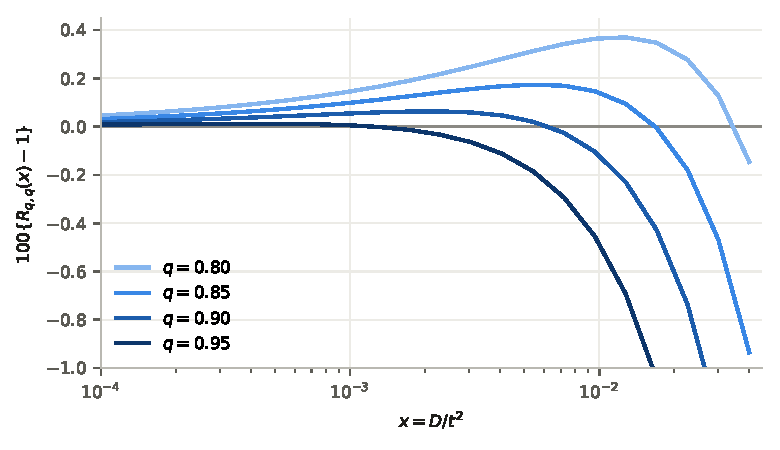
\includegraphics[width=0.7\textwidth]{fig_boundary.pdf}
\caption{Sharp latent radius relative to the noisy threshold, $100\{R_{q,q}(x) - 1\}$, for four coverage levels, computed by grid maximization over the extremal family, which bounds $R_{q,q}$ from below.}
\label{fig:s-boundary}
\end{figure}

\subsection*{The transition: values}

\begin{figure}[t]
\centering
% Alt text: Log-log plot of the leading coefficient against the scaled distance of the mean from the boundary for three levels; each curve is flat up to about 7, 20 and 50, then decays like the reciprocal of the distance, just below a grey upper bound.
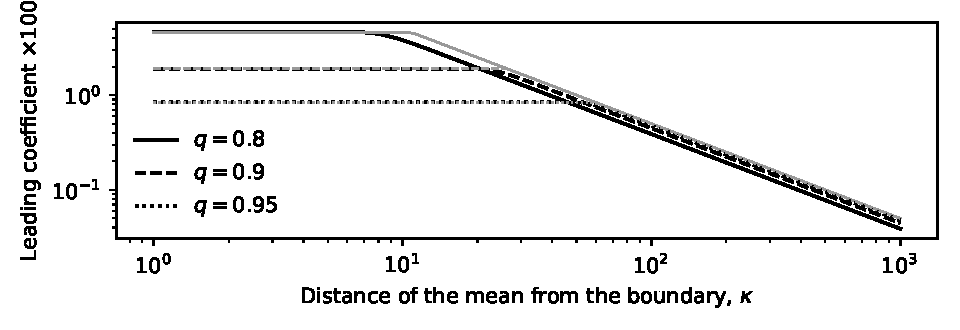
\includegraphics[width=0.9\textwidth]{fig_transition.pdf}
\caption{Leading coefficient $L_q(\kappa)$ of the worst-case radius correction, times $100$, when the mean lies at distance at least $\kappa x^{1/2}$ from the boundary (Theorem~\ref{M-thm:transition}), for $q = 0.8$ (solid), $0.9$ (dashes) and $0.95$ (dots), with the upper bound $\min\{c_q, (\kappa^2 + 1)^{1/2} - \kappa\}$ from Theorems~\ref{M-thm:small} and~\ref{M-thm:mean} (grey). Both axes are logarithmic.}
\label{fig:s-transition}
\end{figure}

The following values are computed in double precision by \texttt{experiments/e32\_centering.py} and are not certified. Table~\ref{tab:s-transition} lists, for $q = 0.8$, $0.9$ and $0.95$, the end $\kappa^*_q$ of the flat part of $L_q$ and the maximizer $u^*$ of $v_q$ at which it is attained, the value of $\kappa$ at which the two upper bounds in Fig.~\ref{fig:s-transition} cross, where $L_q/U_q$ is smallest, with $U_q(\kappa) = \min\{c_q, (\kappa^2 + 1)^{1/2} - \kappa\}$ the upper bound from Theorems~\ref{M-thm:small} and~\ref{M-thm:mean}, that smallest ratio, and the limit $1 - \log(1/q)$ of the ratio as $\kappa \to \infty$.

\begin{table}[h]
\centering
\caption{Transition values, double precision (\texttt{experiments/e32\_centering.py})}
\label{tab:s-transition}
\begin{tabular}{lccc}
\toprule
 & $q = 0.8$ & $q = 0.9$ & $q = 0.95$ \\
\midrule
$\kappa^*_q$ & $6.8118$ & $20.1823$ & $50.0741$ \\
$u^*$ & $0.11328$ & $0.044286$ & $0.018943$ \\
crossing of the upper bounds, $\kappa$ & $10.829$ & $26.221$ & $59.466$ \\
smallest $L_q/U_q$ & $0.770$ & $0.879$ & $0.927$ \\
limit $1 - \log(1/q)$ & $0.777$ & $0.895$ & $0.949$ \\
\bottomrule
\end{tabular}
\end{table}

At $q = 0.9$, $L_q(25) = 0.017393$ and $L_q(50) = 0.0089448$. For the mean-zero laws of Proposition~\ref{prop:centred}, the coefficient with $\beta = 0.2$ and $\ell = 2$ at $q = 0.9$ is $0.0156540$; the expansion is accurate to $6\times10^{-5}$ at $x = 1.3\times10^{-4}$ but fails at $x \approx 1.1\times10^{-3}$, where the noise reaches the end of the support and the threshold may already be shrunk. As a numerical check of the proved bound of Theorem~\ref{M-thm:mean}, including its form with $|E(W)| \le B$, it was evaluated on $642$ laws from the family of Proposition~\ref{prop:centred}, with no violation.

\subsection*{The location of the mean in examples}

Figure~\ref{fig:s-mean} shows the radius correction for laws scaled so that the noisy coverage of $[-1, 1]$ is exactly $0.9$, computed from closed forms by \texttt{experiments/e35\_mean\_location.py}. For the boundary-layer law $W = 1 + x^{1/2}\{b - E_u\}$ at the maximizer $u^*$ of $v_q$, whose mean lies $20.18\,x^{1/2}$ from the boundary, the correction divided by $x^{1/2}$ is $0.019062$ for $x \le 3\times10^{-5}$, equal to $c_{0.9}$. For the same family at the rate with $k_q(u) = 50$ it is $0.008945 = L_{0.9}(50)$. For the fixed mean-zero law of Proposition~\ref{prop:centred} with $\beta\ell = 0.5$ on a unit segment, the correction divided by $x$ is $0.024005$ up to $x = 5\times10^{-5}$, and it turns negative once the noise reaches the end of the support. Larger centred coefficients sit closer to that end: at $\beta\ell = 0.9$ the coefficient is $0.070$ but the quantile lies $0.0011$ from the end, and the correction is positive only for $x$ below about $10^{-7}$. A Gaussian law with mean $1.29\,x^{1/2}$ from the boundary after scaling, $W \sim N(1 - 2x^{1/2}, 0.01x)$ before scaling, needs no correction at all: its radius is $1.16\,x^{1/2}$ below the noisy threshold. A mean near the boundary is necessary for a correction of order $x^{1/2}$, not sufficient.

\begin{figure}[t]
\centering
% Alt text: Log-log plot of the radius correction against the noise ratio for three laws; the two laws with mean near the boundary follow lines of slope one half and the mean-zero law follows a line of slope one.
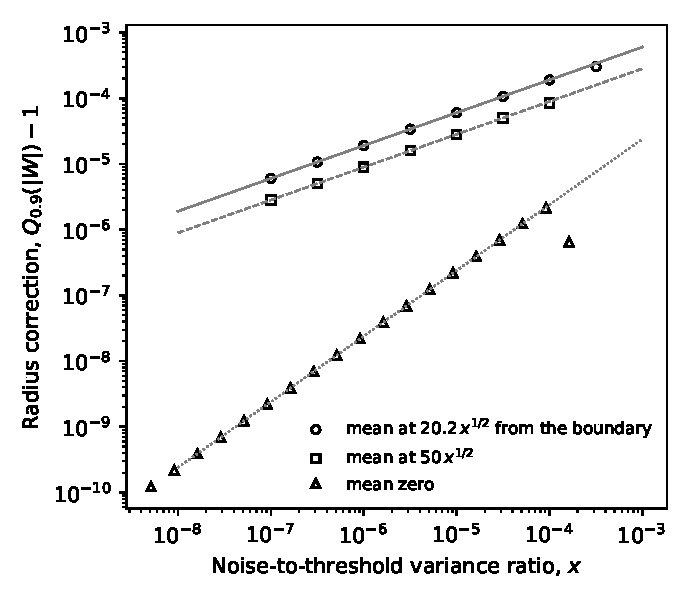
\includegraphics[width=0.6\textwidth]{fig_mean_location.pdf}
\caption{Radius correction $Q_{0.9}(|W|) - 1$ against $x$ on logarithmic axes, for laws with noisy coverage exactly $0.9$: mean at $20.2\,x^{1/2}$ from the boundary (circles), at $50\,x^{1/2}$ (squares) and mean zero (triangles), with $c_{0.9}x^{1/2}$ (solid), $L_{0.9}(50)x^{1/2}$ (dashes) and $0.024\,x$ (dots). Only positive corrections are shown.}
\label{fig:s-mean}
\end{figure}

\subsection*{The limit with $\kappa$ fixed}

Theorem~\ref{M-thm:transition} does not extend to $\kappa$ growing like $x^{-1/2}$, that is, to centred laws; this subsection shows why. Applying the small-$u$ construction to a centred law, that is, $\kappa = x^{-1/2}$, gives in the limit a left exponential tail of rate $1 - \log(1/q)$ whose noise-free central coverage is $q\{1 - \mathrm{e}^{-2 + 2\log(1/q)}\}$, $0.750$ at $q = 0.9$, far below the constraint. So $\{1 - \log(1/q)\}/2$ is not a lower bound for the centred coefficient.

\subsection*{Bi-log-concave laws: scope and examples}

Lemma~\ref{lem:onesided} holds over $\mathcal B$ with the same $c_{p,q}$, and so do the upper bounds of Theorem~\ref{M-thm:small} and Corollary~\ref{M-cor:slack}. The proof of Lemma~\ref{lem:onesided} uses only the concavity of $\log F_Y$ at the $q$-quantile, so its upper bound holds for every $Y$ with $\log F_Y$ concave, and exponential tails are in $\LC$, which gives equality. In the proof of Theorem~\ref{M-thm:small}, $Y = (W - 1)/x^{1/2}$ has $\log F_Y$ concave, and $(-W - 1)/x^{1/2}$ has a concave log distribution function because $\log(1 - F_W)$ is concave and $F_W$ is continuous. The lower bound uses laws in $\LC \subset \mathcal B$.

Proposition~\ref{prop:reduction} and the double-precision upper bounds of \S~\ref{sec:s-cert} use log-concavity of the density; the ball-arithmetic constants do not. Theorems~\ref{M-thm:mean} and~\ref{M-thm:transition}, Lemma~\ref{lem:meanonesided}, Theorem~\ref{M-prop:unknown} and Corollary~\ref{cor:simple} hold over $\mathcal B$, by the facts of \S~\ref{sec:s-prelim}: monotone hazards, the bound $f' \le f^2/F$, and closure under convolution with a log-concave law and under weak limits.

Symmetry alone does not make noisy calibration conservative in $\mathcal B$. The density $f(w) = \{1 + 0.05\cos(2\pi w)\}/2$ on $(-1, 1)$ is in $\mathcal B$, because $\sup|f'| = 0.05\pi < \inf f^2 = 0.2256$ \citep[][Theorem~1]{dumbgen2017}, but it is not unimodal. At $q = 0.7$, $r_0 = Q_q(|W|) \approx 0.7077$ and $f'(r_0) > 0$; since $f'$ is odd, $\partial_s \pr(|W + s^{1/2}Z| \le r_0) = f'(r_0) > 0$ at $s = 0$, so noise raises the coverage and the noisy quantile falls below $r_0$, to $0.707676$ at $s = 10^{-5}$, against $r_0 = 0.707678$. Anderson's comparison needs unimodality. The bound of Theorem~\ref{M-thm:mean} with $E(W) = 0$ holds for this cosine density, recentred to mean zero, and for its version with the cosine phase-shifted by $\pi/2$, at $q = 0.3, 0.7, 0.9$ and $s = 10^{-3}, 0.1, 1$ (test suite).

The bimodal law of Table~\ref{tab:synth}, the mixture $\pi N(m_1, s^2) + (1-\pi)N(m_2, s^2)$ with mean zero, variance one and $(m_2 - m_1)/s = 2.5$, is in $\mathcal B$ by the following lemma. With $\pi = 0.4$ the mixture stays in $\mathcal B$ up to a separation of about $2.59$, while bimodality starts at about $2.443$ (numerical). The parameters are $\pi = 0.4$, $m_1 = -0.94868$, $m_2 = 0.63246$ and $s = 0.63246$.

\begin{lemma}\label{lem:bimodal}
Let $f$ be the density of $\pi N(m_1, s^2) + (1-\pi)N(m_2, s^2)$ with $m_1 < m_2$ and $r = (m_2 - m_1)/s > 2$, let $P(w)$ be the posterior probability of the first component, and let $a < b$ solve $P(a) = \tfrac12 + h$ and $P(b) = \tfrac12 - h$, $h = (1/4 - 1/r^2)^{1/2}$. The mixture is in $\mathcal B$ if $f'F < f^2$ on $[a, m_2]$ and $-f'(1-F) < f^2$ on $[m_1, b]$.
\end{lemma}

\begin{proof}
Since $(\log f)'' = -s^{-2} + P(1-P)r^2s^{-2}$ and $P$ decreases, $f$ is log-concave on $(-\infty, a]$ and on $[b, \infty)$. On $(-\infty, a]$, $F(t) = \int 1(y \le t)f(y)1(y \le a)\,dy$ is the marginal of a log-concave function of $(t, y)$, so $\log F$ is concave there \citep{prekopa1973}; likewise $\log(1-F)$ on $[b, \infty)$. Where $f' \le 0$, in particular on $[m_2, \infty)$, $f'F \le f^2$ is trivial, and where $f' \ge 0$, in particular on $(-\infty, m_1]$, so is $-f'(1-F) \le f^2$. With the two hypotheses, $(\log F)'' \le 0$ and $(\log(1-F))'' \le 0$ on the whole line.
\end{proof}

For the law of Table~\ref{tab:synth} the two hypotheses are proved in Arb ball arithmetic on $128$ boxes, with the ends $a$ and $b$ rounded outward (\texttt{uai.interval.bimodal\_blc\_certificate}, test suite); the largest values of $(f'F - f^2)/f^2$ on $[a, m_2]$ and of $\{-f'(1-F) - f^2\}/f^2$ on $[m_1, b]$ are $-0.141$ and $-0.864$.

\section{Numerical support}\label{sec:s-cert}

Three levels of numerical support are used and kept apart. Certificates in Arb ball arithmetic are proofs. Upper bounds evaluated in double precision with a margin are not interval arithmetic and are labelled numerical. Exploratory searches only propose values and are never used as bounds.

\subsection*{Certificates in ball arithmetic}\label{sec:s-ball}

Every deciding inequality is evaluated in Arb ball arithmetic; floating point only proposes points, balls are converted to doubles with outward rounding, and sums of bounds are formed as balls.
\begin{enumerate}
\item $m_u(b)$ decreases in $b$, and in $u$ because $E_u$ is stochastically decreasing in its rate. Hence $b_u(p)$ is nonincreasing in $u$, and on $[u_0, u_1]$, $b_u(p) - u^{-1}\log(1/q) \le b_{u_0}(p) - u_1^{-1}\log(1/q)$. A ball with $m_u(b) < p$ proves $b_u(p) < b$.
\item For $u \ge u_{\max}$ the value is at most $b_{u_{\max}}(p)$. For small $u$, let $b(u) = \{\log(1/p) + u^2/2 - \log(1 - u^3)\}/u$. Then $\mathrm{e}^{-ub + u^2/2} = p(1 - u^3)$, and the Mills ratio gives $\Phi(-b) \le pu^3$ whenever $\phi\{\log(1/p)/u\} \le p\,u^2\log(1/p)$. This holds on $(0, u_{\min}]$ once it holds at $u_{\min} \le \log(1/p)/2^{1/2}$, because the left side divided by $u^2$ increases there. So $b_u(p) \le b(u)$, and for $p \ge q$ the resulting bound increases in $u$.
\item By Lemma~\ref{lem:onesided}, $c_{p',q'} \le \gamma$ if and only if $1 - q' \ge \varphi_\gamma(1 - p')$, where $\varphi_\gamma(a) = \max[0, \sup_u 1 - \exp\{-u(b_u(1-a) - \gamma)\}]$. Hence $C_{p,q} \le \gamma$ if $\varphi_\gamma(a_L) + \varphi_\gamma(a_R) \le 1 - q$ whenever $a_L + a_R = 1 - p$. Since $\varphi_\gamma$ is nondecreasing, it suffices to check this at the ends of an adaptive partition of $a_L$, with $\varphi_\gamma$ bounded above by the same monotone branch and bound in $u$.
\end{enumerate}
The certificates give $c_{0.8} \in [0.0460730, 0.0460731]$, $c_{0.9} \in [0.0190618, 0.0190619]$, $c_{0.95} \in [0.0084075, 0.0084077]$ and $c_{0.99} \in [0.0013950, 0.0013958]$, $-0.0571845 \le c_{0.9036,0.9} \le C_{0.9036,0.9} \le -0.057$, $-0.1149813 \le c_{0.9068,0.9} \le C_{0.9068,0.9} \le -0.114$, and $C_{p,q} \le 0$ for $(q, p - q) = (0.8, 0.005)$, $(0.9, 0.001)$ and $(0.95, 0.0002)$. Lower bounds $c_{p,q} > 0$ at $p - q = 0.0043$, $0.00079$ and $0.00015$ come from single points $u$, evaluated in ball arithmetic, and $C_{p,q} \ge c_{p,q}$. Hence the smallest slack in Corollary~\ref{M-cor:slack} lies in $(4.3\times10^{-3}, 5.0\times10^{-3}]$, $(7.9\times10^{-4}, 1.0\times10^{-3}]$ and $(1.5\times10^{-4}, 2.0\times10^{-4}]$ at $q = 0.8$, $0.9$ and $0.95$.

For the coverage form of Corollary~\ref{M-cor:slack}, the same certificates give $C_{0.8,0.795} \le 0$, $C_{0.9,0.8991} \le 0$ and $C_{0.95,0.9498} \le 0$, and enclosures give $c_{0.8,0.7954} \ge 7.0\times10^{-4}$, $c_{0.9,0.8992} \ge 4.2\times10^{-4}$ and $c_{0.95,0.9499} \ge 3.0\times10^{-3}$, so by the lower bound of the case $p \ge q$, $R_{p,q'}(x) > 1$ for small $x$ at these pairs (\texttt{experiments/e37\_coverage\_transfer.py}).

Double-precision root finding puts the smallest slack at $4.4\times10^{-3}$, $8.0\times10^{-4}$ and $1.6\times10^{-4}$. In coverage terms: as $x \to 0$ the boundary-layer laws $1 + x^{1/2}\{b_u(q) - E_u\}$, whose noisy coverage tends to exactly $q$, have latent coverage tending to $\mathrm{e}^{-ub_u(q)}$, whose smallest values are $0.79532$, $0.89918$ and $0.94984$ at $q = 0.8$, $0.9$ and $0.95$, attained at $u = 0.140$, $0.0508$ and $0.0210$ (double precision). Calibrating at the noisy level $q$ thus costs at most a few thousandths of latent coverage in these examples, and the certified slack removes the loss. These last values are numerical.

The certificates for the noise classes in \S~\ref{sec:s-general} and for Lemma~\ref{lem:bimodal} follow the same conventions.

\subsection*{Numerical upper bounds of the radius in double precision}

Code and file names that contain `certified' for these quantities, such as \texttt{certified\_R.csv}, \texttt{hetldc\_certified} and \texttt{CertifiedShrinkTable}, are historical: the values are double-precision upper bounds, not ball-arithmetic certificates.

By the symmetry $W \mapsto -W$ of the kernel and of $|W|$ it suffices to treat $\beta \ge 0$. Write a member of $\mathcal F$ with $\beta \ge 0$ as $W = b - Y$, where $Y$ has density proportional to $\mathrm{e}^{-\beta y}$ on $[0,\ell]$. The ends of the family are included: $\ell = 0$ or $\beta = \infty$ gives a point mass and $\ell = \infty$ an exponential tail. For slopes $\beta' > \beta$ the likelihood ratio $\mathrm{e}^{-(\beta'-\beta)y}$ is decreasing, so $Y_{\beta'}$ lies below $Y_\beta$ in likelihood-ratio order, and for lengths $\ell < \ell'$ truncation gives $F_\ell \ge F_{\ell'}$. Thus $W$ is stochastically increasing in $\beta$ and $b$ and decreasing in $\ell$. On a box of parameters let $W_{\rm lo}$ and $W_{\rm hi}$ be the stochastically smallest and largest corners. Since $\pr(W + e \le \pm 1)$ and $\pr(W \le y)$ are expectations of decreasing functions of $W$, every law in the box satisfies
\[
\pr(|W+e| \le 1) \le \pr(W_{\rm lo} + e \le 1) - \pr(W_{\rm hi} + e \le -1),\qquad \pr(|W| \le s) \ge \pr(W_{\rm hi} \le s) - \pr(W_{\rm lo} \le -s).
\]
The density bound $\pr(|W+e| \le 1) \le 2\sup f_W = 2\beta/(1 - \mathrm{e}^{-\beta\ell})$ is also available. A box whose first bound is below $p$, or whose second bound is at least $q$, contains no law that violates $R_{p,q}(x) \le s$, and a branch and bound over boxes certifies $R_{p,q}(x) \le s$. The location is confined to $[-1 + x^{1/2}\Phi^{-1}(p), b_{\max}]$. The lower end holds because $W \le b$. For the upper end let $k_0 = 7x^{1/2}$. The density of $W$ increases towards $b$, so $\pr(|W| \le 1 + k_0) \le \rho_0/(1 + \rho_0)$ with $\rho_0 = (2 + 2k_0)/(b - 1 - k_0)$, and $\pr(|e| > k_0) = 2\Phi(-7)$; $b_{\max}$ is the smallest $b$ with $\rho_0/(1 + \rho_0) + 2\Phi(-7) < p$, beyond which no law is feasible. The parameters $\beta, \ell \in [0,\infty]$ are compactified.

\begin{proposition}\label{prop:continuity}
For all $x, h \ge 0$, $R_{p,q}(x + h) \le R_{p,q}(x) + c_q h^{1/2}$.
\end{proposition}

\begin{proof}
If $W$ is feasible at noise level $x + h$, then $W + h^{1/2}Z'$, with $Z' \sim N(0,1)$ independent of $(W, Z)$, is log-concave and feasible at level $x$. So $s = Q_q(|W + h^{1/2}Z'|) \le R_{p,q}(x)$, and Theorem~\ref{M-thm:small} at scale $s$ gives $Q_q(|W|) \le s + c_q h^{1/2}$.
\end{proof}

We computed numerical upper bounds of $R_{p,0.9}$ for $p = 0.9$, $0.9036$ and $0.9068$ on $0.002 \le x \le 0.366$ with step $5\times10^{-4}$, using Proposition~\ref{prop:continuity} between grid points. Here $0.9068$ and $0.9036$ are the order-statistic levels $p_k$ of $K = 110$, $k = 105$ at $\delta = 0.05$ and $\delta = 0.04$; the latter is used in \S~\ref{sec:s-hetero}.

These bounds rest on double-precision evaluation of the closed forms and are not interval arithmetic. Boxes are cleared with a margin of $10^{-9}$. In the test suite the closed forms agree with $30$-digit quadrature at random points with $10^{-4} \le x \le 1.5$, $10^{-4} \le \ell \le 20$ or $\ell = \infty$ and $10^{-3} \le \beta\ell \le 10^{3}$, which cover the ranges where boxes are evaluated, including the mixture kernels of Table~\ref{tab:synth}, whose largest ratio $D_i/T^2$ is about $1.25$. The largest error found was $1.1\times10^{-12}$ for $x \le 0.37$ and $2.5\times10^{-11}$ above.

For $0.05 \le x \le 0.3$ the bound exceeds a feasible value by at most a relative $3\times10^{-4}$ for $p = 0.9$ and $10^{-3}$ for $p = 0.9068$. The branch and bound fails only just before the feasibility edges, near $x = 0.370$ for $p = 0.9$, on $0.3585 \le x \le 0.3615$ for $p = 0.9036$ and on $0.352 \le x \le 0.3545$ for $p = 0.9068$; there Proposition~\ref{prop:continuity} from the last grid point gives $R_{0.9,0.9}(x) \le 0.132$. Below $x = 0.01$ the lookup also uses Theorem~\ref{M-thm:small} and its $p \ge q$ form, which are within $0.3\%$ of a feasible value there (Fig.~\ref{fig:s-certified}). At $q = 0.9$ the numerical bounds fall below $1$ from $x = 0.013$ on, with the continuity margin $c_{0.9}(5\times10^{-4})^{1/2} \approx 4.3\times10^{-4}$ keeping them below $1$ between grid points, and reach $0.973$ at $x = 0.05$.

\begin{figure}[t]
\centering
% Alt text: Line plot of numerical upper bounds of the sharp radius against the noise ratio; the bounds lie above one only for small noise ratios and fall well below the shape-free bound.
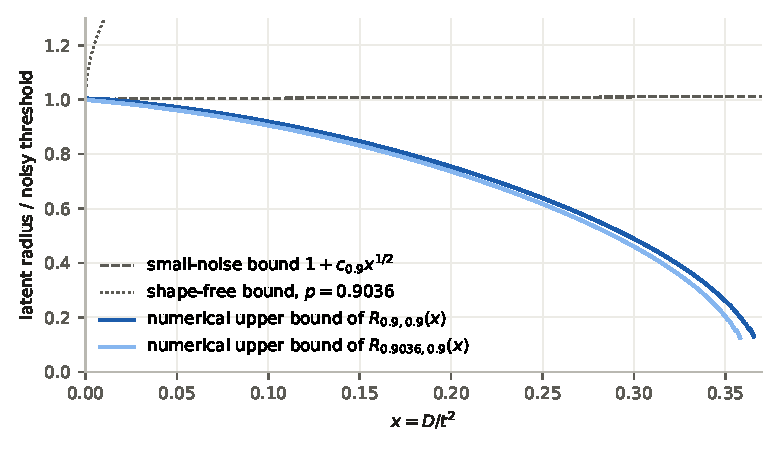
\includegraphics[width=0.7\textwidth]{fig_certified.pdf}
\caption{Numerical upper bound of the sharp radius $R_{p,0.9}(x)$ for $p = 0.9$ and for the order-statistic level $p = 0.9036$ ($\delta = 0.04$), with the small-noise bound of Theorem~\ref{M-thm:small} and the shape-free bound $1 + x^{1/2}z_{1-(p-q)/2}$, which follows from $|W| \le |V| + |e|$.}
\label{fig:s-certified}
\end{figure}

\subsection*{Exploratory searches}

Grid maximization over the extremal family, as in Fig.~\ref{fig:s-boundary}, gives lower bounds of $R_{q,q}$; grid values below $1$ do not show that shrinking is safe. This two-dimensional computation over slope and length, and an independent differential-evolution search over the three-parameter family, agree to $1.5\times10^{-13}$ at all $73$ tabulated values of $x \ge 0.006$ (numerical). The search is used only for $x \ge 0.006$: it evaluates the constraint by Gauss--Legendre quadrature, which is inaccurate for steep slopes at small $x$, and at $x = 0.001$ it returned $1.027$, above the bound $1.0006$ of Theorem~\ref{M-thm:small}.

\section{Heterogeneous and estimated noise variances}\label{sec:s-hetero}

\subsection*{Heterogeneous known variances}

This section gives the rules of \S~\ref{M-sec:hetero}, which use the noise variances $D_i$ when they are known, with Gaussian noise. They are an extension: the main results need neither the variances nor the noise law.

\emph{The computed radius.} Let $T = |V|_{(k)}$ and let
\[
\bar g(w) = K^{-1}\sum_{i=1}^K \pr(|w + e_i| \le T)
\]
be the average noisy kernel at $T$. By Proposition~\ref{prop:beta}, with probability at least $1 - \delta$ over calibration samples, $\int \bar g\,dG \ge p_k$, the $\delta$-quantile of the ${\rm Beta}(k, K+1-k)$ distribution; the proof needs $k \ge Kp_k + 1$, which holds for the ranks used here. Let $R^{\rm mix}$ be defined by \eqref{M-eq:R} with the constraint $\int \bar g\,dG \ge p_k - \omega$, where $\omega$ bounds the error from compressing the $D_i$ to a few support points. By Proposition~\ref{prop:reduction}, which holds for this kernel, the computed radius $T R^{\rm mix}$ covers the latent target with probability at least $q$, given the data, on an event of probability at least $1 - \delta$, for every log-concave $G$. This guarantee is for the exact $R^{\rm mix}$; the implementation computes a numerical upper bound on it in double precision, not a certificate.

In the heterogeneous rule, $\omega$ bounds, for each data set, the sup-norm error of the average kernel after compressing the $D_i$ to $32$ support points: the maximum over a grid of spacing $h = 10^{-3}$ plus $Mh^2/8$, with $M$ a bound on the second derivative; it was about $2\times10^{-4}$. For each data set a numerical upper bound of $R^{\rm mix}$ is computed by the box bounds, which hold term by term for a mixture kernel, and the shape-free bound is used if the branch and bound fails.

Replacing the average kernel by the kernel of a single variance is not safe. With the mean variance plugged in, the radius is $1.4\%$ too short at mean $x = 0.2$ with lognormal spread $1$ (numerical). The smallest variance also fails: take $W = b - E_2$ with $b = 1.0435647$ and noise an equal mixture of $N(0, 10^{-8})$ and $N(0, 5\times10^{-4})$. The noisy coverage of $[-1, 1]$ exceeds $0.9$, while the radius $1 + c_{0.9}10^{-4}$ given by the smaller variance covers $W$ with probability $0.89977$; this was checked in $192$-bit ball arithmetic.

\subsection*{A known lower bound on the variances}

\begin{corollary}\label{cor:simple}
Let $G \in \mathcal B$ and $k \ge Kp_k + 1$. If $D_i \ge D_{\min}$ for all $i$ and $C_{p',q} < 0$ for some $p'$ with $q \le p' \le p_k$, then $s = \max\{0, T + C_{p',q}D_{\min}^{1/2}\}$ satisfies $\pr_{\mathcal D}\{\pr(|W_{\rm new}| \le s \mid \mathcal D) \ge q\} \ge 1 - \delta$, whether or not the $D_i$ are otherwise known.
\end{corollary}

\begin{proof}
On the event of Proposition~\ref{prop:beta}, some $i$ has $\pr(|W + e_i| \le T) \ge p_k \ge p'$, and the bound of \S~\ref{M-sec:slack} at $x = D_i/T^2$ gives $Q_q(|W|) \le T + C_{p',q}D_i^{1/2} \le T + C_{p',q}D_{\min}^{1/2}$.
\end{proof}

At $q = 0.9$, $K = 110$ and $\delta = 0.05$, where $p_k = 0.906806$, ball arithmetic gives $C_{0.9068,0.9} \le -0.114$, hence $s = T - 0.114 D_{\min}^{1/2}$, the shrunk threshold of Table~\ref{tab:synth}.

\subsection*{Estimated variances}

Suppose the $D_i$ are unknown and estimates $\hat D_i$ are available that are independent of the scores, as for the sample means and variances of normal unit data. The order-statistic event of Proposition~\ref{prop:beta} involves the scores only. Let $\mathcal A_\eta$ be an event determined by the $\hat D_i$ with $\pr(\mathcal A_\eta) \ge 1 - \eta$. For a vector $D = (D_1, \ldots, D_K)$ of variances and a threshold $t$, let $\bar g_{D,t}(w) = K^{-1}\sum_i \pr(|w + D_i^{1/2}Z| \le t)$ be the average kernel. For a kernel $u$, let $R_{p,q}[u]$ be the radius \eqref{M-eq:R} with the constraint replaced by $\int u\,dG \ge p$, in units in which the threshold is $1$, and write $R^{\rm mix}_{p,q}(x_1, \ldots, x_K) = R_{p,q}[\bar g_{x,1}]$, the radius for the average kernel with variances $x_i = D_i/t^2$ at threshold $1$.

\begin{lemma}\label{lem:dominate}
Let $G \in \LC$. Suppose that on $\mathcal A_\eta$ a continuous kernel $u_t$, vanishing at $\pm\infty$, satisfies $u_t \ge \bar g_{D,t}$ pointwise for every $t > 0$. Then $s = T\,R_{p_k,q}[u_T]$ covers a new latent residual with probability at least $q$, conditionally on the data, with probability at least $1 - \delta - \eta$. If $\mathcal D_\eta$ is a confidence set with $\pr(D \in \mathcal D_\eta) \ge 1 - \eta$, the same holds for $s = T\sup_{d \in \mathcal D_\eta} R^{\rm mix}_{p_k,q}(d/T^2)$. With a compressed kernel, $p_k$ is replaced by $p_k - \omega$ as in \S~\ref{sec:s-hetero}.
\end{lemma}

\begin{proof}
On both events, $\int u_T\,dG \ge \int \bar g_{D,T}\,dG \ge p_k$, and Proposition~\ref{prop:reduction} applies to $u_T$. The union bound gives $1 - \delta - \eta$, with no independence between the two events needed.
\end{proof}

\begin{lemma}\label{lem:scale}
For $\lambda \ge 1$, $R^{\rm mix}_{p,q}(\lambda x_1, \ldots, \lambda x_K) \le \lambda^{1/2} R^{\rm mix}_{p,q}(x_1, \ldots, x_K)$.
\end{lemma}

\begin{proof}
If $W$ is feasible at $\lambda x$, then $U = \lambda^{-1/2}W$ satisfies the constraint at threshold $\lambda^{-1/2} \le 1$, hence at threshold $1$, so $Q_q(|W|) = \lambda^{1/2}Q_q(|U|) \le \lambda^{1/2}R^{\rm mix}_{p,q}(x)$.
\end{proof}

A confidence box for all $K$ variances needs level $1 - \eta/K$ per area and is useless with one or two degrees of freedom. Survey practice instead models variances through a few parameters, as generalized variance functions do. In the simplest such model $D_i = \sigma^2 a_i$ with known $a_i$, for instance $a_i = 1/n_i$, and the pooled estimate satisfies $\nu\hat\sigma^2/\sigma^2 \sim \chi^2_\nu$ with $\nu = \sum_i(n_i - 1)$. The confidence set is the segment $\{\sigma^2 a : \ell \le \sigma^2 \le h\}$. Lemma~\ref{lem:scale} covers the supremum over it by finitely many points without assuming that $R$ is monotone in $\sigma^2$: for $\ell = s_0 < \cdots < s_m = h$,
\[
\sup_{\ell \le \sigma^2 \le h} R^{\rm mix}_{p_k,q}(\sigma^2 a/T^2) \le \max_j\,(s_{j+1}/s_j)^{1/2}\,U_j, \qquad U_j \ge R^{\rm mix}_{p_k,q}(s_j a/T^2).
\]
Plugging in the lower end $\ell$ alone would not be justified, since $R$ can increase with the noise level (Theorem~\ref{M-thm:small}).

In the simulations below most radii are grid values, which are lower bounds of $R^{\rm mix}$ and so carry no guarantee; the rule with numerical upper bounds, as Lemma~\ref{lem:dominate} requires, was run on a subset. Areas have $n_i$ normal units, so $D_i = \sigma_i^2/n_i$ and the within-area variances are independent of the direct estimates; $K = 110$, mean $D = 0.577$, and $100$ replications per setting and law (normal, Laplace, truncated Laplace). The rule uses $\delta = 0.04$ and $\eta = 0.01$, split as $0.009$ below and $0.001$ above the pooled interval for $\sigma^2$, and needs $18$ grid points on average. The radii reported use converged grid values at those points; for the first $30$ data sets of every setting and law ($270$ in all) the rule was rerun with numerical upper bounds $U_j$ at every grid point. The branch and bound succeeded for every data set, and the half-width grew by $0.14\%$ on average and by at most $1.0\%$, at about $3.6$ minutes per data set on one core.
\begin{enumerate}
\item With $n_i \in \{2, 3\}$, $\nu \approx 165$, the rule is $6.3$--$6.5\%$ shorter than noisy conformal calibration and $2.9$--$3.0\%$ longer than the known-variance rule at the same level, which is $9.0$--$9.1\%$ shorter than noisy conformal calibration. With $n_i \in \{5, \ldots, 10\}$, $\nu \approx 740$, the figures are $7.1$--$7.7\%$ and $1.6$--$1.7\%$. Relative to the known-variance rule at $\delta = 0.05$, which needs no budget for the variances and meets the same final target, $62$--$63\%$ and $73$--$74\%$ of its gain survive. Reliability of the rule with grid values was at least $0.98$; with numerical upper bounds, on the $30$ data sets per setting, it was at least $0.967$.
\item The supremum over the interval exceeded the value at its lower end by $0.2\%$.
\item When the within-area variances differ, with lognormal spread $0.5$, the common-variance model is wrong and no guarantee applies; the rule was still reliable, at least $0.99$, and $5.9$--$6.5\%$ shorter than noisy conformal calibration.
\item Without pooling, with each area's variance estimated from $\nu$ own degrees of freedom, a kernel envelope built from area-wise intervals and a binomial bound on the number of misses is $31$--$40\%$ longer than noisy conformal calibration at $\nu = 2$, within $1.3\%$ of it at $\nu = 50$, and $4.7$--$5.0\%$ and $6.6$--$7.2\%$ shorter at $\nu = 200$ and $1000$ ($30$ replications per law; grid values). Whether a better area-wise construction exists is open.
\end{enumerate}

\section{The Markov rule}\label{sec:s-shapefree}

\begin{proposition}\label{prop:shapefree}
Let $\bar g$ be a kernel that is symmetric, continuous, strictly decreasing in $|w|$ and tends to $0$ as $|w| \to \infty$, with $m = \bar g(0)$, and suppose that $qm < p < m$. Over all laws $G$ on the real line with $\int \bar g\,dG \ge p$, the supremum of $Q_q(|W|)$ is the radius $r$ that solves $\bar g(r) = (p - qm)/(1 - q)$.
\end{proposition}

\begin{proof}
Let $\tau = (p - qm)/(1-q) \in (0, m)$. Since $m - \bar g(W) \ge 0$, Markov's inequality gives $\pr\{\bar g(W) < \tau\} \le \{m - p\}/(m - \tau) = 1 - q$, and $\bar g(W) < \tau$ exactly when $|W| > r$, so $Q_q(|W|) \le r$. Conversely, for small $\epsilon > 0$ put mass $q - \epsilon$ at $0$ and mass $1 - q + \epsilon$ at the point $w_\epsilon > 0$ with $\bar g(w_\epsilon) = \{p - (q - \epsilon)m\}/(1 - q + \epsilon)$. This law meets the constraint with equality, has $Q_q(|W|) = w_\epsilon$, and $w_\epsilon \to r$ as $\epsilon \to 0$.
\end{proof}

The average kernel of \S~\ref{sec:s-hetero} satisfies these conditions, so for a fixed rank the Markov rule of Table~\ref{tab:synth} is the smallest radius that the single order-statistic constraint allows without a shape assumption. With $1$ in place of $\bar g(0)$ it contains the bound of \citet{guille2024}. It is not a bound on procedures that use several thresholds or tune the rank on independent data, as LatentCP \citep{zheng2026} can.

\section{A shifted new residual}\label{sec:s-shift}

\begin{proposition}\label{prop:shift}
Let $W$ be log-concave with standard deviation $\varsigma$, let $\pr(|W| \le t) \ge q'$ and $|\Delta| \le \rho\varsigma$. Then $\pr(|W + \Delta| \le t) \ge q' - \rho$. Conversely, for symmetric unimodal noise and noisy coverage $p$, there are log-concave $W$ for which the noisy threshold has latent coverage $\lambda_{\mathcal E}(p)$ and $\pr(|W + \rho\varsigma| \le t) \to \lambda_{\mathcal E}(p)\mathrm{e}^{-\rho}$.
\end{proposition}

\begin{proof}
A shift by $\Delta > 0$ moves the window $[-t, t]$ to $[-t - \Delta, t - \Delta]$, which loses at most the mass of $(t - \Delta, t]$, at most $\Delta \sup f$. For a log-concave density $\varsigma \sup f \le 1$, with equality for the exponential law \citep{bobkov2015}, so the loss is at most $\rho$. For the converse let $q_0 = \lambda_{\mathcal E}(p)$, $b = u^{-1}\log(1/q_0)$ and $W = t + b - E_u$, so that $\varsigma = 1/u$ and $\pr(W \le t) = \pr(E_u \ge b) = q_0$, and let the noise be uniform on $[-r/u, r/u]$ with $r$ the maximizer of Theorem~\ref{M-thm:classes}(i) at $q_0$. As $ut \to \infty$ the left end does not matter, the latent coverage tends to $q_0$ and, by scaling, the noisy coverage to $E\{\min(1, q_0 \mathrm{e}^{-rU})\} = \Psi_{\mathcal E}(q_0) = p$, with $U$ uniform on $[-1, 1]$; a shift by $\rho/u$ gives $\pr(W + \rho/u \le t) = \pr(E_u \ge b + \rho/u) = q_0 \mathrm{e}^{-\rho}$. The loss $q_0(1 - \mathrm{e}^{-\rho}) = q_0\rho + O(\rho^2)$ shows that the linear order of the bound cannot be improved; it does not attain the coefficient one.
\end{proof}

At $q = 0.9$ the guaranteed latent coverage of noisy coverage $0.9$ under symmetric unimodal noise is thus between $0.8881$ and $0.8892$ for $\rho = 0.01$, and between $0.798$ and $0.813$ for $\rho = 0.1$. Measured relative to $t$ rather than to $\varsigma$, a shift has no nontrivial bound: point masses just inside the threshold satisfy every noisy constraint.

\section{Simulations and an application}\label{sec:s-sim}

Table~\ref{tab:s-sims} lists the experiments of this section and the claim each supports. The laws of Table~\ref{tab:synth} and of Table~\ref{M-tab:sameinfo} are far from the extremal laws of \S\S~\ref{M-sec:general}--\ref{M-sec:mean}, which is why the guarantees are conservative there; the stress test uses an extremal law.

\begin{table}[h]
\centering
\caption{Experiments and the claims they support}
\label{tab:s-sims}
\footnotesize
\begin{tabular}{>{\raggedright\arraybackslash}p{0.32\textwidth}>{\raggedright\arraybackslash}p{0.58\textwidth}}
\toprule
experiment & claim \\
\midrule
rules with the same information & Table~\ref{M-tab:sameinfo}: width of the ranks of Theorem~\ref{M-prop:unknown} when the noise is unknown \\
stress test at the extremal law & Proposition~\ref{M-prop:fail}: without the raise the latent reliability falls as $K$ grows \\
rules with known variances & \S~\ref{sec:s-hetero}: the computed radius and the shrunk threshold \\
analytic rules, $2000$ data sets & how conservative the guarantees are for these laws \\
sensitivity to a shared latent law & the Discussion: the guarantees need one latent law shared by all units \\
oracle-matched widths & the width needed for a guarantee, separated from the shape of the interval \\
LatentCP and deconvolution & comparison with the methods of \citet{zheng2026} and \citet{cohen2025} \\
school districts & behaviour on survey data with estimated variances, which no guarantee covers \\
\bottomrule
\end{tabular}
\end{table}

\subsection*{Rules with the same information}

The design is given in \S~\ref{M-sec:numerical} (\texttt{experiments/e43\_same\_information.py}). Each noise law is scaled to variance $D_i$: uniform on $[-(3D_i)^{1/2}, (3D_i)^{1/2}]$, Laplace with scale $(D_i/2)^{1/2}$, $t_3$ multiplied by $(D_i/3)^{1/2}$, and $D_i^{1/2}(E_1 - 1)$ for the centred exponential. Latent coverage given the data is computed from the latent distribution function. Extra width is $2T$ for a rule divided by $2T$ for the usual rank, computed setting by setting.

\subsection*{A stress test at the extremal law}

\texttt{experiments/e38\_stress.py} uses the boundary-layer law $W = \theta - x^{1/2}E_u$ with $x = 10^{-4}$. The rate $u = 0.0508$ minimizes the limiting latent coverage $\mathrm{e}^{-ub_u(q)}$ at $q = 0.9$; it is not the radius maximizer $u^*$ of \S~\ref{sec:s-shape}. The location $\theta$ makes the population noisy coverage $\pr(|W + e| \le 1)$ equal to $0.9$. The noise variances are equal, or lognormal as in Table~\ref{tab:synth} and scaled to mean $x$. The population latent coverage is then $0.89918$ with equal variances, within $10^{-4}$ of the certified bound $0.8991$ of Corollary~\ref{M-cor:slack}, so the worst case at this noise level lies in $[0.8991, 0.89918]$, and $0.89959$ with unequal ones. The raised rank below is that of Theorem~\ref{M-prop:unknown} for Gaussian noise. Conditional latent coverage is exact; $\delta = 0.05$; $20000$ data sets for $K = 110$ and $1000$ and $10000$ for $K = 10^4$.

\begin{table}[h]
\centering
\caption{Stress test, equal variances: mean conditional latent coverage and reliability (standard errors in parentheses), target $0.9$ and $0.95$}
\label{tab:s-stress}
\begin{tabular}{llccc}
\toprule
$K$ & rank & $k$ & mean latent coverage & reliability \\
\midrule
$110$ & marginal & $100$ & $0.9004\ (0.0002)$ & $0.531\ (0.004)$ \\
 & usual and raised & $105$ & $0.9503\ (0.0002)$ & $0.966\ (0.001)$ \\
$1000$ & marginal & $901$ & $0.89931\ (0.00007)$ & $0.482\ (0.004)$ \\
 & usual & $916$ & $0.91483\ (0.00007)$ & $0.943\ (0.002)$ \\
 & raised & $917$ & $0.91588\ (0.00007)$ & $0.954\ (0.001)$ \\
$10^4$ & marginal & $9001$ & $0.89918\ (0.00003)$ & $0.395\ (0.005)$ \\
 & usual & $9050$ & $0.90419\ (0.00003)$ & $0.922\ (0.003)$ \\
 & raised & $9060$ & $0.90522\ (0.00003)$ & $0.961\ (0.002)$ \\
\bottomrule
\end{tabular}
\end{table}

The usual rank keeps its noisy guarantee, with noisy reliability $0.952$ and $0.954$ at $K = 1000$ and $10^4$, but loses the latent one, by $4$ and $10$ standard errors; the raised rank of Theorem~\ref{M-prop:unknown} restores it. The marginal rank has mean latent coverage below $0.9$ once $K \ge 1000$, by $0.0008$ at $K = 10^4$, the deficit of Corollary~\ref{M-cor:slack}. With unequal variances the reliabilities are $0.948$ and $0.960$ at $K = 1000$, and $0.936$ and $0.968$ at $K = 10^4$, for the usual and the raised rank. At $K = 110$ the two ranks coincide and the order-statistic level $0.9068$ leaves ample room. These simulations agree with the exact reliability $\pr\{{\rm Bin}(K, H(r_q)) \le k - 1\}$ of Proposition~\ref{M-prop:fail}, with $H(r_q) = 0.90080$: $0.943$ and $0.954$ at $K = 1000$, $0.918$ and $0.958$ at $K = 10^4$ for the usual and the raised rank. Figure~\ref{fig:s-reliability} extends the exact values to $K = 10^6$ (\texttt{experiments/e40\_exact\_reliability.py}); the usual rank falls to $0.790$ at $K = 10^5$ and $0.151$ at $K = 10^6$, the marginal rank to $0.004$, while the raised rank stays above $0.95$ and reaches $0.989$ at $K = 10^6$. On the grid of $15$ values of $K$ from $30$ to $298$ in \texttt{results/exact\_reliability.csv} ($K = 30, 36, 43, 51, 61, 73, 87, 103, 110, 123, 147, 175, 209, 249, 298$) the usual rank has exact reliability at least $0.9459$, at $K = 298$, so its shortfall from $0.95$ is at most $0.0041$ there.

\begin{figure}[t]
\centering
% Alt text: Line plot of latent reliability against calibration sample size on a logarithmic axis; the raised rank stays near or above 0.95 throughout, the usual rank declines from about 0.95 to 0.15 at one million, and the marginal rank declines from about 0.55 to near zero.
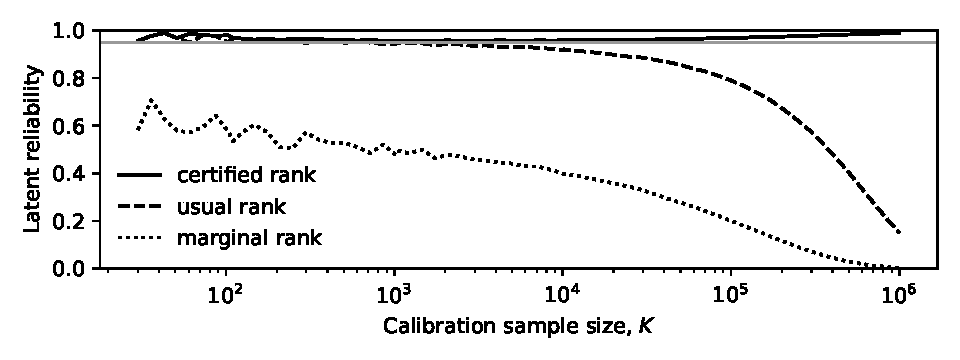
\includegraphics[width=0.8\textwidth]{fig_reliability.pdf}
\caption{Exact latent reliability at the boundary-layer law of the stress test, equal variances with standard deviation $1\%$ of the threshold, for the raised rank of Theorem~\ref{M-prop:unknown} (solid), the usual high-probability rank (dashes) and the marginal rank (dots), $\delta = 0.05$; grey, the target $0.95$.}
\label{fig:s-reliability}
\end{figure}

So the slack is not an artefact of the proofs: without it the latent guarantee fails at this law once the calibration sample is large enough for the order statistic to resolve a coverage difference of $10^{-3}$. The effect needs small noise and a latent law with a sharp edge just beyond the threshold, here $2\%$ beyond it.

\subsection*{Rules with known variances}

The rules of \S~\ref{sec:s-hetero}, which use the known noise variances, are compared with the noisy threshold, a Fay--Herriot interval and the Markov rule of \S~\ref{sec:s-shapefree}. The target is $\pr_{\mathcal D}\{\pr(W_{\rm new} \in C \mid \mathcal D) \ge 0.9\} \ge 0.95$, with $K = 110$, $\var(W) = 1$ and Gaussian noise with heterogeneous variances $D_i = 0.577\,L_i/E(L_i)$, $L_i$ lognormal with log-scale $0.7$. Latent residuals, all with mean zero, are drawn directly; conditional coverage given each data set is exact, and reliability is estimated from $150$ data sets per law. Besides four standard log-concave laws we use a truncated exponential law in $\mathcal F$, a bimodal law in $\mathcal B$ but not in $\LC$, and a $t_3$ law outside $\mathcal B$. We compare the noisy threshold at rank $105$, the shrunk threshold and the computed radius of \S~\ref{sec:s-hetero}, a Fay--Herriot tolerance interval adapted from \citet{chatterjee2008}, and the Markov rule, the radius $r$ with $\bar g(r) = \{p_k - q\bar g(0)\}/(1 - q)$, the smallest the single constraint allows without a shape assumption (\S~\ref{sec:s-shapefree}), at its best rank, $107$.

\begin{table}[h]
\centering
\caption{Rules with known variances: reliability, times $100$, and mean width (in parentheses); target $95$}
\label{tab:synth}
\small
\begin{tabular}{lccccc}
\toprule
latent law & Markov & Fay--Herriot & noisy threshold & shrunk & computed \\
\midrule
normal & 100 (5.92) & 96 (3.93) & 100 (4.96) & 100 (4.90) & 98 (4.45) \\
Laplace & 100 (6.29) & 93 (3.96) & 100 (5.15) & 100 (5.09) & 99 (4.66) \\
centred gamma & 100 (6.16) & 100 (3.95) & 100 (4.97) & 100 (4.90) & 100 (4.45) \\
truncated Laplace & 100 (5.89) & 85 (3.89) & 100 (4.93) & 100 (4.87) & 97 (4.42) \\
truncated exponential & 100 (6.17) & 95 (3.93) & 100 (5.06) & 100 (4.99) & 100 (4.55) \\
bimodal ($\mathcal B$ only) & 100 (5.77) & 100 (4.01) & 100 (4.87) & 100 (4.81) & 99 (4.35) \\
$t_3$ (outside $\mathcal B$) & 100 (5.70) & 97 (3.80) & 100 (4.66) & 100 (4.60) & 98 (4.09) \\
\bottomrule
\end{tabular}

\medskip
\parbox{0.95\textwidth}{\footnotesize Noisy threshold, $T$ at rank $105$; shrunk, $\max\{0, T - 0.114D_{\min}^{1/2}\}$ with $D_{\min} = \min_i D_i$; computed, $T R^{\rm mix}$; centred gamma with shape $2$; truncated exponential, density proportional to $\mathrm{e}^{4w}$ on $[0,1]$, standardized; bimodal, the mixture of Lemma~\ref{lem:bimodal}; widths are full widths. The Markov rule is guaranteed for every law; under the bimodal law the noisy and shrunk thresholds are guaranteed and the computed radius is exploratory; under $t_3$ the noisy threshold is guaranteed by Anderson's theorem. Standard errors are at most $2.9$ for reliabilities and $0.08$ for widths. Reliabilities are rounded: the Fay--Herriot reliability under the truncated exponential law is $0.947$, below the target.}
\end{table}

The rules with a guarantee reached the target for every law in their class, and the computed radius did so also under the bimodal and $t_3$ laws, for which it has none. The computed radius was $9.5$--$12\%$ shorter than the noisy threshold and $24$--$28\%$ shorter than the Markov rule. The Fay--Herriot interval was $7$--$15\%$ shorter than the computed radius but fell short of the target under three laws, as detailed below.

Conditional coverage is computed from closed-form latent distribution functions. With $150$ data sets the binomial standard error of a reliability is $0.018$ at $0.95$ and at most $0.029$ at the lowest reliability observed, $0.847$; for instance $145/150 = 0.967$ has the $95\%$ binomial interval $[0.924, 0.989]$. The computed radius uses the order-statistic level $p_k = 0.9068$ of $\delta = 0.05$. The branch and bound returned a numerical upper bound of $R^{\rm mix}$ for every one of the $1050$ data sets, at relative tolerance $10^{-3}$ in $671$, $3\times10^{-3}$ in $363$ and $10^{-2}$ in $16$, so the shape-free fallback was never used. With the mean variance in a single Gaussian kernel, which is not a valid plug-in, the numerical radius at level $p_k$ is $2.9$--$3.2\%$ shorter than at level $p = q$, so most of the gain over a $p = q$ calibration comes from the order-statistic level.

The Markov rule was run at every fixed rank $106$--$110$; rank $107$ is reported because it is best on average over the first four laws, which favours the comparison rule.

The Fay--Herriot interval falls short of the target under the Laplace law by about $1.3$ standard errors, under the truncated exponential law, with reliability $0.947$, by $0.2$, and under the truncated Laplace law, with reliability $0.847$, by about $5.8$. The Fay--Herriot tolerance interval is our adaptation of the parametric bootstrap of \citet{chatterjee2008} to an intercept-only model: the bootstrap $(1-\delta)$-quantile of the multiplier each refit needs to cover $N(\hat\mu, \hat A)$ with probability $0.9$. The latent residuals are drawn directly, with no fitted centre, and the mean noise variance $0.577$ matches the ratio of design to model variance in the application below.

\subsection*{Reliability of the analytic rules with $2000$ data sets}

The noisy threshold, Corollary~\ref{cor:simple} and the Markov rule need no numerical optimization, so \texttt{experiments/e36\_analytic\_reliability.py} reran them on $2000$ fresh data sets for each of the seven laws of Table~\ref{tab:synth}. Every rule reached conditional coverage $0.9$ in all $2000$ data sets for every law, so each reliability has Clopper--Pearson $95\%$ interval $[0.998, 1]$, including the $t_3$ law, outside $\mathcal B$. Mean conditional coverage was $0.969$--$0.992$ for the noisy threshold, $0.968$--$0.991$ for Corollary~\ref{cor:simple} and $0.984$--$0.998$ for the Markov rule, and the $5\%$ quantile of conditional coverage was at least $0.947$, $0.945$ and $0.968$.

\subsection*{Sensitivity to a shared latent law}

Theorem~\ref{M-prop:unknown} assumes that the calibration residuals and the new one share a law $G$, independent of the noise variances. \texttt{experiments/e39\_sensitivity.py} uses the design of Table~\ref{tab:synth} with $2000$ data sets for the normal, centred gamma and truncated exponential laws and two kinds of departure: residual standard deviation proportional to $D_i^{1/2}$ or $D_i^{-1/2}$, standardized to variance one, with the new area drawing its variance from the same population; and a new area whose residual is shifted by $\pm0.2$ or $\pm0.5$ latent standard deviations.
\begin{enumerate}
\item Averaged over the new area's variance, the dispersion departures left the reliability of the noisy threshold and of Corollary~\ref{cor:simple} at $1$, with mean coverage $0.967$--$0.976$, against $0.968$--$0.984$ without departure. Conditionally on the new area's variance this fails: at the $10\%$ quantile of the variances, when dispersion falls with the variance, and at the $90\%$ quantile, when it rises, mean coverage was $0.918$--$0.942$ and reliability as low as $0.75$. Neither case is covered by Theorem~\ref{M-prop:unknown}, which assumes one law independent of the variances: averaged over new areas the reliability was kept in these designs, but not given a new area's variance.
\item Shifts of $\pm0.2$ changed mean coverage by at most $0.010$, with reliability $1$; shifts of $\pm0.5$ lowered it by up to $0.027$, to $0.941$ under the truncated exponential law, with reliability at least $0.977$ and $5\%$ quantile of conditional coverage $0.908$.
\item At the boundary-layer law of the stress test, with $K = 110$ and $20000$ data sets, the noisy threshold has reliability $0.969$; shifting the new residual towards the edge by $0.1$ latent standard deviations, $2\%$ of the threshold, lowered mean coverage to $0.860$ and reliability to $0.035$, and by $0.25$ to $0.741$ and $0$, while shifts away from the edge raised coverage above $0.999$.
\end{enumerate}
The robustness in the first two items does not come from the margin between $p_k$ and $q$; near an extremal law a systematic difference between sampled and unsampled areas is not tolerated.

\subsection*{Oracle-matched widths}

This experiment compares interval shapes at equal reliability. Besides marginal noisy conformal calibration and Fay--Herriot intervals it includes the log-concave rule, the noisy threshold at rank $105$ rescaled by the sharp radius $R_{0.9,0.9}$ evaluated at a lower confidence bound for a common noise variance. With seven latent shapes, common and heterogeneous noise and $2000$ data sets per setting, each rule's width was rescaled by a single factor, chosen with knowledge of the latent law, to reach reliability $0.95$ exactly. At matched reliability, marginal noisy conformal calibration was shortest in $12$ of the $14$ settings and the Fay--Herriot tolerance interval in the other $2$; relative to noisy conformal calibration the Fay--Herriot tolerance interval was $3.1\%$ shorter to $12.1\%$ longer and the log-concave rule $4.5$--$11.5\%$ longer (\texttt{results/conditional\_synth\_exact\_matched.csv}). The log-concave rule with its guarantee was a median $15\%$ (range $9$--$33\%$) wider than its own oracle-matched width, and the Fay--Herriot tolerance interval a median $6\%$ (range $-3$ to $16\%$). So the advantage of the log-concave rule over noisy conformal calibration lies in obtaining a latent guarantee cheaply, not in a better interval shape.

\subsection*{Comparison with LatentCP and deconvolution}

\texttt{experiments/e34\_competitors.py} runs the following rules on the $600$ data sets of the first four laws of Table~\ref{tab:synth}; widths are relative to the computed radius. For the other three laws only the two analytic rules were run.
\begin{enumerate}
\item LatentCP \citep{zheng2026}, single level with $\gamma = \alpha/2$, has a marginal guarantee. Its latent set depends on the new unit's noise variance, which an unsampled area does not have; we draw it from the distribution that generated the $D_i$, $400$ draws per data set, and average coverage and width over the draws. It was $16$--$18\%$ longer, with mean coverage $0.976$--$0.990$ and reliability $1.0$. The tuned single-level and two-level versions, tuned on half the data, were $15$--$25\%$ longer. A PAC version with a binomial rank, our adaptation, was $39$--$58\%$ longer.
\item The deconvolution threshold of \citet{cohen2025}, with the mixture kernel in place of their homoscedastic kernel, collapses at $K = 110$ with their bin width $0.01$: most bins are empty and the masked fit gives mean coverage $0.32$--$0.44$. With bin width $0.2$ and the empty bins fitted as zeros it had mean coverage $0.88$--$0.90$, reliability $0.45$--$0.67$ and width $22$--$30\%$ shorter; it has no latent guarantee.
\item The noisy threshold of Theorem~\ref{M-prop:unknown} was $10.5$--$11.7\%$ longer and Corollary~\ref{cor:simple} $9.1$--$10.2\%$ longer, both with reliability $1.0$.
\end{enumerate}
The tuning grids of LatentCP and the scan step $0.01$ of the deconvolution threshold are our choices; the original papers do not fix them for this setting.

\subsection*{School districts}

In the finite population \texttt{apipop} \citep{lumley2004}, $110$ of $325$ school districts are used for training and $110$ for calibration, with $2$ or $3$ schools sampled per district. Coverage is the share of the remaining $105$ districts that are covered. Design variances are estimated with $1$--$2$ degrees of freedom and plugged in as known by every rule, a case that no guarantee covers. Over four conditions of $120$ replications, the reliability of the heterogeneous rule, the computed radius with the average kernel, was $0.942$--$0.992$, of the mean-variance rule, which plugs the mean variance into a single Gaussian kernel, $0.983$--$1.000$ and of the Fay--Herriot interval $0.908$--$0.992$, below target in two conditions. The heterogeneous rule at level $p_k$ was $0.8$--$5.2\%$ shorter than the mean-variance rule calibrated at level $p = q$, mostly because of the level, and $10$--$16\%$ longer than the Fay--Herriot interval.

\section{Reproducibility}\label{sec:s-code}

All computations are in the public repository \url{https://github.com/kunhailP/latent-coverage-noisy-thresholds}; the submitted version is the tag \texttt{biometrika-submission}. The core routines are in \texttt{src/uai}: closed forms and the transition coefficient in \texttt{extremal.py}, the box bounds in \texttt{certify.py}, ball arithmetic in \texttt{interval.py}, the noise-class constants and certificates in \texttt{noise\_classes.py}, and the procedures in \texttt{procedures.py} and \texttt{estimated.py}. The test suite, run by \texttt{make test}, checks the constants, the counterexamples, the centring bounds, the convexity of $\Psi$ for symmetric unimodal noise and the closed forms of Proposition~\ref{M-prop:latentshape}, and the \texttt{Makefile} lists the command that produces each group of results. Table~\ref{tab:s-code} maps results to scripts in \texttt{experiments} and to output files in \texttt{results}.

\begin{table}[h]
\centering
\caption{Results, scripts and output files}
\label{tab:s-code}
\footnotesize
\begin{tabular}{p{0.40\textwidth}p{0.25\textwidth}p{0.29\textwidth}}
\toprule
result & script & output \\
\midrule
Theorem~\ref{M-thm:classes}, noise classes & \texttt{e41\_noise\_classes.py} & \texttt{noise\_classes.json} \\
Proposition~\ref{M-prop:latentshape}, unimodal latent laws & \texttt{e42\_unimodal\_boundary.py} & printed \\
Table~\ref{M-tab:sameinfo}, rules with the same information & \texttt{e43\_same\_information.py} & \texttt{same\_information.csv} \\
Lemma~\ref{lem:onesided}, Corollary~\ref{M-cor:slack}: $c_{p,q}$, $C_{p,q}$, slack & \texttt{e27\_interval\_constants.py} & \texttt{interval\_constants.json} \\
Coverage form of Corollary~\ref{M-cor:slack} & \texttt{e37\_coverage\_transfer.py} & \texttt{coverage\_transfer.json} \\
Numerical upper bounds of the radius & \texttt{e24\_certified\_table.py}, \texttt{e25\_certified\_ldc.py} & \texttt{certified\_R.csv}, \texttt{certified\_ldc\_summary.csv} \\
Centring and transition values, Fig.~\ref{fig:s-transition} & \texttt{e32\_centering.py}, \texttt{fig\_transition.py} & \texttt{centering.json} \\
Location of the mean, Fig.~\ref{fig:s-mean} & \texttt{e35\_mean\_location.py}, \texttt{fig\_mean\_location.py} & \texttt{mean\_location.csv} \\
Table~\ref{tab:synth}, rules with known variances & \texttt{e20\_hetldc\_synth.py}, \texttt{e31\_shape\_free.py} & \texttt{hetldc\_synth\_summary.csv}, \texttt{shape\_free\_summary.csv} \\
Analytic rules, $2000$ data sets & \texttt{e36\_analytic\_reliability.py} & \texttt{analytic\_reliability\_summary.csv} \\
Stress test, Table~\ref{tab:s-stress} & \texttt{e38\_stress.py} & \texttt{stress\_summary.csv} \\
Proposition~\ref{M-prop:fail}, Fig.~\ref{fig:s-reliability} & \texttt{e40\_exact\_reliability.py} & \texttt{exact\_reliability.csv} \\
Sensitivity to a shared latent law & \texttt{e39\_sensitivity.py} & \texttt{sensitivity\_summary.csv}, \texttt{sensitivity\_stress.csv} \\
Oracle-matched widths & \texttt{e15\_e12\_exact.py} & \texttt{conditional\_synth\_exact\_matched.csv} \\
LatentCP and deconvolution & \texttt{e34\_competitors.py} & \texttt{competitors\_summary.csv} \\
Estimated variances & \texttt{e29\_estimated\_scale.py}, \texttt{e30\_areawise\_variance.py} & \texttt{estimated\_scale\_summary.csv}, \texttt{areawise\_variance\_summary.csv} \\
School districts & \texttt{e21\_hetldc\_apipop.py} & \texttt{hetldc\_apipop\_summary.csv} \\
Shape-free rule & \texttt{e31\_shape\_free.py} & \texttt{shape\_free\_summary.csv} \\
Lemma~\ref{lem:bimodal}, bimodal law & \texttt{uai.interval.bimodal\_blc\_certificate} & test suite \\
\bottomrule
\end{tabular}
\end{table}

The analytic rules of Theorem~\ref{M-prop:unknown} and Corollary~\ref{cor:simple} are \texttt{noisy\_threshold\_halfwidth} and \texttt{simple\_shrink\_halfwidth} in \texttt{procedures.py}, and \texttt{certified\_rank} returns the rank for Gaussian noise; \texttt{hetldc\_certified} gives the computed radius, while \texttt{hetldc\_halfwidth} returns a grid value, a lower bound of $R^{\rm mix}$, and is not a guaranteed radius.


\section{An open problem: the extremal log-concave noise law}\label{sec:s-open}

This section is not used by any result. It records a partial argument towards the conjecture that the centred exponential law attains $\Psi_{\mathcal E}$ for mean-zero log-concave noise, which Theorem~\ref{M-thm:classes}(ii) leaves open; the certified bounds there do not depend on it.

Since $h(y) = q \mathrm{e}^{-\max(y, \ell)}$, with $X = -\epsilon$ and $c = -\ell$,
\[
\Psi_{\mathcal E}(q) = q \sup E\{e^{\min(X, c)}\},
\]
the supremum over mean-zero log-concave $X$, and the conjectured extremal law is $X = \sigma(1 - E_1)$, with $E_1$ standard exponential. Laws bounded above by $c$ are covered analytically. If $X \le s$ almost surely with $0 < s \le c$, the log-density of $X$ minus the affine log-density of $s(1 - E_1)$ is concave on $(-\infty, s]$, so the difference of densities changes sign at most twice; with equal masses and means, the difference of distribution functions changes sign once, from negative to positive, so $X$ is smaller than $s(1 - E_1)$ in the convex order. As $x \mapsto \mathrm{e}^{\min(x, c)}$ is convex on $(-\infty, s]$, $E\{e^{\min(X, c)}\} \le E\{e^{\min(s(1 - E_1), c)}\}$. The open case is a law with mass above $c$, where the objective is not convex; the extremal law lies there, with $\sigma = 0.11777 > c = 0.10536$ at $q = 0.9$, and choosing the scale of the comparison law freely gives crossing patterns from which no sign follows.

\bibliographystyle{biometrika}
\bibliography{refs}

\end{document}